\chapter{Geodesics in Schwarzschild spacetime}
\label{s:ges}
\index{geodesic!in Schwarzschild spacetime}

\minitoc

\section{Introduction}

We have already investigated some geodesics in Schwarzschild spacetime in
Chap.~\ref{s:sch}, namely
the radial null geodesics (Sec.~\ref{s:sch:rad_null_geod}).
Here, we perform a more extensive study. In particular we investigate timelike
geodesics, which are of primordial physical importance, since they represent
orbits of planets or stars around the black hole or worldlines of
intrepid observers freely falling into the black hole.

\section{Geodesic motion}

Let $\Li$ be a geodesic\footnote{The definition and basic properties of geodesics
are recalled in Appendix~\ref{s:geo}.} of Schwarzschild spacetime
$(\M,\w{g})$. We shall assume that $\Li$ is causal, i.e. either timelike or null\footnote{As
shown in Sec.~\ref{s:geo:def}, a geodesic cannot be partly timelike and partly
null.}. It therefore can be considered as the worldline
of some particle $\mathscr{P}$, either massive
($\Li$ timelike) or masseless ($\Li$ null).


\subsection{First integrals of motion} \label{s:ges:fiom}

The Schwarzschild spacetime $(\M,\w{g})$ is static and spherically symmetric; the
Killing vector $\w{\xi}$ associated with the staticity (cf. Sec.~\ref{s:sch:static_spher})
and the Killing vector $\w{\eta}$ associated with the rotation symmetry along any
axis, give birth to two conserved quantities along $\Li$:
\begin{greybox}
The scalar products
\begin{subequations}
\label{e:ges:conserved_quantities}
\begin{align}
& \encadre{E := - \w{\xi}\cdot \w{p} = - \w{g}(\w{\xi},\w{p}) } \label{e:ges:conserved_energy} \\
& \encadre{L := \w{\eta}\cdot \w{p} = \w{g}(\w{\eta},\w{p}) } , \label{e:ges:conserved_angu_mom}
\end{align}
\end{subequations}
where $\w{p}$ is the 4-momentum of particle
$\mathscr{P}$ (cf. Sec.~\ref{s:fra:worldlines}),
are constant along the geodesic $\Li$.
The scalar $E$ is called $\mathscr{P}$'s
\defin{conserved energy}\index{conserved!energy}\index{energy!conserved --}
or \defin{energy at infinity}\index{energy!at infinity},
while $L$ is called $\mathscr{P}$'s \defin{conserved angular momentum}\index{conserved!angular momuntum}\index{angular momentum!conserved --}
or \defin{angular momentum at infinity}\index{angular momentum!at infinity}.
\end{greybox}
\begin{proof}
The 4-momentum $\w{p}$ is a tangent vector associated with an affine parameter
of $\Li$, i.e. it obeys the geodesic equation (\ref{e:fra:p_geodesic}).
The constancy of $E$ and $L$ follow then from the generic property (\ref{e:geo:g_xi_v_const})
of geodesics in presence of a spacetime symmetry.
\end{proof}
In coordinates $(t,r,\th,\ph)$ adapted to the spacetime symmetries,
i.e. coordinates such that $\w{\xi} = \wpar_t$ and $\w{\eta}=\wpar_\ph$, like the Schwarzschild-Droste
coordinates or the Eddington-Finkelstein ones, one can rewrite
(\ref{e:ges:conserved_quantities})
in terms of the components $p_t = g_{t\mu} \, p^\mu$ and $p_\ph = g_{\ph\mu} \, p^\mu$
of the 1-form $\uu{p}$ associated to $\w{p}$ by metric duality:
\begin{subequations}
\begin{align}
& E = - p_t \\
& L = p_\ph
\end{align}
\end{subequations}
Indeed, in such a coordinate system, $\xi^\mu =  \delta^\mu_{\ \, t}$
and $\eta^\mu = \delta^\mu_{\ \, \ph}$, so that $E = -g_{\mu\nu} \, \xi^\mu p^\nu = -g_{t\nu} \, p^\nu = -p_t$
and $L = g_{\mu\nu} \, \eta^\mu p^\nu = g_{\ph\nu} \, p^\nu = p_\ph$.


It is worth stressing that $E$ is not a genuine energy, i.e. it is not
an energy measured by some observer. Indeed the latter is defined by
Eq.~(\ref{e:fra:E_obs}), which resembles Eq.~(\ref{e:ges:conserved_energy})
but differs from it by $\w{\xi}$ not being a unit vector in general:
$\w{\xi}\cdot\w{\xi} \not = -1$. In other words, $\w{\xi}$ cannot
be interpreted as the 4-velocity of some observer, so that the quantity
$E$ defined by (\ref{e:ges:conserved_energy}) cannot be a \emph{physically measured}
particle energy. It is only in the asymptotic region, where $\w{\xi}\cdot\w{\xi} = g_{tt}
\rightarrow -1$, that $\w{\xi}$ is an eligible 4-velocity, hence the name
\emph{energy at infinity}. Note that this name is commonly used, even in the
particle $\mathscr{P}$ never visits the asymptotic region.
Similarly, $L$ is not some (component of a) genuine angular momentum. Only in the
asymptotic region do we have
\be \label{e:ges:ell_asympt}
    L \simeq g_{\ph\ph} \, p^\ph \simeq r^2\sin^2\ph \, p^\ph \simeq r^2\sin^2\theta \, P^\ph
    \simeq r\sin\th \, P^{(\ph)} ,
\ee
where $P^{(\ph)}$ is the azimuthal component of the momentum $\w{P}$ of particle $\mathscr{P}$
as measured by an asymptotic inertial observer (cf. Sec.~\ref{s:fra:measure}), i.e.
the component of $\w{P}$ along $\w{e}_{(\ph)}$ in the orthonormal basis $(\w{e}_{(r)}, \w{e}_{(\th)}, \w{e}_{(\ph)})$, with $\w{e}_{(\ph)} = (r\sin\th)^{-1} \wpar_\ph$.
In view of (\ref{e:ges:ell_asympt}), we may say that $L$ is the angular momentum
about the symmetry axis $\th=0$ that an inertial observer would attribute to
particle $\mathscr{P}$ if the latter would move close to him.

From its very definition, Eq.~(\ref{e:ges:conserved_energy}), $E$ is
a positive
quantity as soon as the geodesic $\Li$ has some part in $\M_{\rm I}$, i.e.
some part with $r>2m$:
\begin{greybox}
\be \label{e:ges:E_positive_M_I}
    \Li \cap \M_{\rm I} \not= \varnothing \quad \Longrightarrow \quad E > 0 .
\ee
\end{greybox}
\begin{proof}
In $\M_{\rm I}$, the Killing vector $\w{\xi}$ is timelike and future-directed.
The 4-momentum $\w{p}$ is either timelike or null and always future-directed.
By Eq.~(\ref{e:fra:scalar_caus1}), one has then necessarily $\w{\xi}\cdot\w{p} < 0$; hence Eq.~(\ref{e:ges:conserved_energy})
implies $E > 0$ in $\M_{\rm I}$. Since $E$ is constant along $\Li$, it
follows that $E > 0$ everywhere.
\end{proof}
\begin{remark}
If the geodesic $\Li$ is confined to $\M_{\rm II}$, i.e. to the black hole
region (cf. Sec.~\ref{s:sch:BH}),
where $\w{\xi}$ is spacelike (cf. Sec.~\ref{s:sch:SD_domain}),
it is possible to have $E \leq 0$, since the
scalar product of $\w{p}$ with a spacelike vector can take any value.
\end{remark}
\begin{remark}\label{r:ges:L_any_sign}
The Killing vector $\w{\eta}$ being always spacelike,
the scalar product $\w{g}(\w{\eta},\w{p})$ can a priori take any real value, and
thus there is no constraint
on the sign of $L$.
\end{remark}

To be specific, let us describe Schwarzschild spacetime in terms of the
Schwarzschild-Droste coordinates $(t,r,\th,\ph)$ introduced in Sec.~\ref{s:sch:solving_EE}.
Without any loss of generality, we may choose these coordinates so that
at $t=0$, the particle $\mathscr{P}$ is located in the equatorial plane $\th=\pi/2$ and
the spatial projection of the worldline $\Li$ lies in that plane, i.e. $\w{p}$ has
no component along $\wpar_\th$:
\be
    \w{p} \stackrel{t=0}{=} p^t \wpar_{t} + p^r \wpar_r + p^\ph \wpar_\ph .
\ee
Now, if for $t>0$, the geodesic $\Li$ were departing from $\th=\pi/2$, this
would constitute some breaking of spherical symmetry, making a difference
between the ``Northern'' hemisphere and the ``Southern'' one.
Hence\footnote{More rigorously, Eq.~(\ref{e:ges:pth_zero}) can
be derived from the geodesic equation (\ref{e:fra:p_geodesic}): given
the expression of the Christoffel symbols of $\w{g}$ in Schwarzschild-Droste
coordinates (cf. Sec.~\ref{s:sam:Kottler_solution}), Eq.~(\ref{e:fra:p_geodesic})
yields \[\frac{\D p^\th}{\D\lambda} +\frac{2}{r}  p^r p^\th - \sin\th\cos\th \left( p^\ph \right)^2 = 0,\] where $\lambda$ is the affine parameter of $\Li$ associated with $\w{p}$,
so that $p^\th=\D\th/\D\lambda$. Whatever the values of $r(\lambda)$,
$p^r(\lambda)$ and $p^\ph(\lambda)$,
the solution of this ordinary differential equation with the initial conditions $p^\th=0$ and
$\cos\th=0$ is $p^\th=0$ for all values of $\lambda$.} $\Li$
must stay at $\th=\pi/2$, which implies
\be \label{e:ges:pth_zero}
    \encadre{p^\th = 0} .
\ee
We conclude that
\begin{greybox}
A geodesic $\Li$ of Schwarzschild spacetime is necessarily confined to a timelike hypersurface.
Without any loss of generality, we can choose Schwarzschild-Droste coordinates $(t,r,\th,\ph)$
such that this hypersurface is the ``equatorial hyperplane'' $\th=\pi/2$.
Then the component $p^\th$ of the 4-momentum of the particle having $\Li$ as worldline
vanishes identically [Eq.~(\ref{e:ges:pth_zero})].
\end{greybox}

Let us denote by $\mu$ the mass of particle $\mathscr{P}$, with possibly
$\mu=0$ if $\mathscr{P}$ is a photon. The scalar square of the 4-momentum $\w{p}$ is
then [cf. Eq.~(\ref{e:fra:def_mass})]
\be \label{e:ges:p2_mu2}
    \w{g}(\w{p},\w{p}) = - \mu^2 .
\ee

\subsection{Equations of motion and generic properties} \label{s:ges:eq_to_be_solved}

Contemplating Eqs.~(\ref{e:ges:conserved_energy}), (\ref{e:ges:conserved_angu_mom}),
(\ref{e:ges:pth_zero}) and (\ref{e:ges:p2_mu2}), we realize that we have
four first integral of motions. The problem is then completely integrable.
More specifically, let $\lambda$ be the affine parameter along the geodesic
$\Li$ associated with the 4-momentum $\w{p}$ (cf. Eq.~(\ref{e:geo:v_dxdlambda}):
\be \label{e:ges:def_lambda}
    \w{p} = \frac{\D\w{x}}{\D\lambda} ,
\ee
where  $\D\w{x}$ is the infinitesimal displacement along $\Li$ corresponding
to the parameter change $\D\lambda$. Note that $\lambda$ is dimensionless.
In terms of the components with respect to Schwarzschild-Droste coordinates,
this yields
\be \label{e:ges:comp_4_momentum}
    \dot{t} := \frac{\D t}{\D\lambda} = p^t,\qquad
    \dot{r} := \frac{\D r}{\D\lambda} = p^r,\qquad
    \dot{\th} := \frac{\D \th}{\D\lambda} = p^\th,\qquad
    \dot{\ph} := \frac{\D \ph}{\D\lambda} = p^\ph .
\ee
In the present case, where $\th(\lambda)=\pi/2$, we have of course $\dot{\th}=0$,
in agreement with Eq.~(\ref{e:ges:pth_zero}).
Given the components (\ref{e:sch:Schwarz_metric_SD}) of Schwarzschild metric
with respect to the Schwarzschild-Droste coordinates,
Eq.~(\ref{e:ges:conserved_energy}) can be written as
\[
    E = - g_{t\mu} p^\mu = - g_{tt} p^t = - g_{tt} \dot{t}
    = \left(1 - \frac{2m}{r} \right) \dot{t} ,
\]
hence
\be \label{e:ges:dot_t}
    \encadre{\frac{\D t}{\D \lambda} = E \left(1 - \frac{2m}{r} \right) ^{-1} }.
\ee
Similarly, Eq.~(\ref{e:ges:conserved_angu_mom}) becomes
\[
    L = g_{\ph\mu} p^\mu = g_{\ph\ph} p^\ph  = g_{\ph\ph} \dot{\ph}
        = r^2 \sin^2\th \, \dot{\ph} .
\]
Since $\th=\pi/2$, we get
\be \label{e:ges:dot_ph}
    \encadre{\frac{\D\ph}{\D\lambda} = \frac{L}{r^2} } .
\ee
We have already noticed that the sign of $L$ is unconstrained (Remark~\ref{r:ges:L_any_sign} on p.~\pageref{r:ges:L_any_sign}). The above equation
shows that it corresponds to the increase ($L>0$) or decrease $(L<0)$
of $\ph$ along the geodesic $\Li$. In other words, we deduce from Eq.~(\ref{e:ges:dot_ph})
that
\begin{greybox}
Along any timelike or null geodesic of Schwarzschild spacetime,
the azimuthal coordinate $\ph$ is either constant ($L=0$)
or increases (resp. decreases) monotically ($L>0$) (resp. $L<0$).
\end{greybox}

The last unexploited first integral of motion is Eq.~(\ref{e:ges:p2_mu2}); it
yields
\[
   - \left( 1 - \frac{2m}{r} \right) (\dot{t})^2 +
   \left( 1 - \frac{2m}{r} \right) ^{-1}  (\dot{r})^2
   + r^2 (\dot{\th})^2 + r^2 \sin^2\th (\dot{\ph})^2  = - \mu^2 .
\]
Using (\ref{e:ges:dot_t}), (\ref{e:ges:dot_ph}), as well as
$\dot{\th}=0$ and $\th=\pi/2$, we get
\[
    -  E^2 \left(1 - \frac{2m}{r} \right) ^{-1}
    +  \left( 1 - \frac{2m}{r} \right) ^{-1}  (\dot{r})^2
    +  \frac{L^2}{r^2} = - \mu^2 ,
\]
which can be recast as
\be \label{e:ges:dot_r_square}
    \encadre{ \left( \frac{\D r}{\D \lambda} \right) ^2
        - \frac{2 \mu^2 m}{r} + \frac{L^2}{r^2}
         \left( 1 - \frac{2m}{r} \right) = E^2 - \mu^2 } .
\ee
To summarize, we may say that the geodesic motion in Schwarzschild spacetime is governed by
Eqs.~(\ref{e:ges:dot_t}), (\ref{e:ges:dot_ph}) and (\ref{e:ges:dot_r_square}),
where $r=r(\lambda)$ and $\mu$, $E$ and $L$ are constants.
This constitutes a system of 3 differential equations for the 3 unknown
functions $t(\lambda)$, $r(\lambda)$ and $\ph(\lambda)$.
We observe
that Eq.~(\ref{e:ges:dot_r_square}) is decoupled from the other two equations.
The task is then to first solve this equation for $r(\lambda)$ and to inject
the solution into Eqs.~(\ref{e:ges:dot_t}) and (\ref{e:ges:dot_ph}), which
can then be integrated separately.

A constraint to keep in mind is that the 4-momentum vector $\w{p}$, whose
components are related to the solution $(t(\lambda), r(\lambda), \ph(\lambda))$
by Eq.~(\ref{e:ges:comp_4_momentum}), has to be a future-directed causal vector.
In $\M_{\rm I}$, as we have seen above, this is guaranteed by choosing $E > 0$
[cf. Eq.~(\ref{e:ges:E_positive_M_I})]. In $\M_{\rm II}$, a future-directed
timelike vector is $-\wpar_r$ (cf. Sec.~\ref{s:sch:time_orientation}).
According to Eq.~(\ref{e:fra:scalar_caus1}), we have then
$\w{p}$ future-directed iff $-\wpar_r\cdot\w{p} < 0$, i.e. iff
\[
    \left(\frac{2m}{r} - 1  \right) ^{-1} p^r < 0  .
\]
Since $2m/r - 1 > 0$ in $\M_{\rm II}$, this is equivalent to $p^r < 0$, i.e.
to $\D r/\D\lambda < 0$. Hence
\begin{greybox}
In the black hole region $\M_{\rm II}$, i.e. for $r<2m$,
the solution $r(\lambda)$ of Eq.~(\ref{e:ges:dot_r_square})
must be a strictly decreasing function of $\lambda$.
\end{greybox}
Actually, we recover the result stated for any causal worldline (not necessarily
a geodesic) in Sec.~\ref{s:sch:time_orientation}.

\begin{remark}
We have derived the system of Eqs.~(\ref{e:ges:dot_t}), (\ref{e:ges:dot_ph}) and (\ref{e:ges:dot_r_square}) without invoking explicitly the
famous \emph{geodesic equation}\index{geodesic!equation}\index{equation!geodesic --}, i.e.
Eq.~(\ref{e:geo:eq_geod}) in Appendix~\ref{s:geo}.
This is because we had enough
first integrals of the second-order differential equation
(\ref{e:geo:eq_geod})
to completely reduce it to
a system of first order equations.
\end{remark}

In what follows, we discuss separately the resolution of
the system (\ref{e:ges:dot_t})-(\ref{e:ges:dot_r_square}) for timelike geodesics
(Sec.~\ref{s:ges:timelike}) and for null ones (Sec.~\ref{s:ges:null}).


\section{Timelike geodesics} \label{s:ges:timelike}

\subsection{Effective potential} \label{s:ges:eff_pot_timelike}

When the geodesic $\Li$ is timelike, it is natural to use the proper time $\tau$
as an affine parameter along it, instead of the parameter $\lambda$ associated
with the 4-momentum $\w{p}$. Since the tangent vector associated with $\tau$
is the 4-velocity $\w{u}$ (cf. Sec.~\ref{s:fra:massive_part}) and $\w{p}$ and $\w{u}$ are related by
Eq.~(\ref{e:fra:p_m_u}): $\w{p} = \mu \, \w{u}$, we get
$\D\w{x}/\D\lambda = \mu \, \D\w{x}/\D\tau$, from which we infer the relation
between $\tau$ and $\lambda$:
\be
    \tau = \mu \lambda ,
\ee
up to some additive constant. This is
of course a special case of the generic relation (\ref{e:geo:affine_transf})
between two affine parameters of the same geodesic.
Equation~(\ref{e:ges:dot_r_square}) becomes then
\be \label{e:ges:1d_motion_timelike}
    \encadre{ \frac{1}{2} \left( \frac{\D r}{\D \tau} \right) ^2
        + V_{\ell}(r) = \frac{\veps^2 - 1}{2} } ,
\ee
where
\be \label{e:ges:V_eff_timelike}
     \encadre{V_{\ell}(r) := - \frac{m}{r} + \frac{\ell^2}{2 r^2}
     \left( 1 - \frac{2 m}{r} \right)}
\ee
and $\veps$ and $\ell$ are respectively the
\defin{specific conserved energy}\index{specific!conserved!energy}
and \defin{specific conserved angular momentum}\index{specific!conserved!angular momuntum}
of particle $\mathscr{P}$:
\be \label{e:ges:def_eps_ell}
  \encadre{ \veps := \frac{E}{\mu} = - \w{\xi}\cdot \w{u}}\qquad\mbox{and}\qquad
  \encadre{ \ell :=  \frac{L}{\mu} = \w{\eta}\cdot\w{u}} ,
\ee
where $\w{u}$ is the 4-velocity of $\mathscr{P}$ and the second equalities
result from definitions (\ref{e:ges:conserved_quantities})
and the relation $\w{p} = \mu \, \w{u}$ [Eq.~(\ref{e:fra:p_m_u})].
Note that $\veps$ is dimensionless (in units $c=1$) and that it shares the
same positiveness property (\ref{e:ges:E_positive_M_I}) as $E$,
namely $\veps$ is positive as soon as the timelike geodesic $\Li$ has some part
in $\M_{\rm I}$, i.e. some part with $r>2m$:
\begin{greybox}
\be \label{e:ges:eps_positive_M_I}
    \Li \cap \M_{\rm I} \not= \varnothing \quad \Longrightarrow \quad \veps > 0 .
\ee
\end{greybox}
On the contrary, $\ell$ can be either positive, zero or negative, depending
on the variation of $\ph$ along $\Li$, as was already noticed above for $L$.

We note that Eq.~(\ref{e:ges:1d_motion_timelike}) has the shape of the
first integral of the
1-dimensional motion of a non-relativist particle in the potential
$V_{\ell}$ (called hereafter the \defin{effective potential}\index{effective!potential!timelike geodesic}), the term $1/2 \, (\D r/\D\tau)^2$ being interpreted as
the kinetic energy per unit mass, $V_{\ell}(r)$ as the potential
energy per unit mass and the constant right-hand side $(\veps^2-1)/2$ as the total
mechanical energy per unit mass.
\begin{remark} \label{r:ges:V_eff_Newt}
The effective potential (\ref{e:ges:V_eff_timelike}) differs from its
non-relativistic (Newtonian) counterpart only by the factor $1-2m/r$ instead of
$1$. This difference plays an important role for small values of $r$,
leading to some orbital instability, as we shall see in Sec.~\ref{s:ges:circular_orbits}.
\end{remark}

In $\M_{\rm I}$, where the Killing vector $\w{\xi}$ is timelike,
we may introduce the \defin{static observer}\index{static!observer}
$\Obs$, whose 4-velocity $\w{u}_{\Obs}$ is colinear to $\w{\xi}$:
\be
    \w{u}_{\Obs} = \left( 1 - \frac{2m}{r} \right) ^{-1/2} \, \w{\xi} ,
\ee
the proportionality coefficient ensuring that $\w{u}_\Obs\cdot\w{u}_\Obs=-1$
given that $\w{\xi}\cdot\w{\xi} = g_{tt} = - (1-2m/r)$.
We have then, from (\ref{e:ges:def_eps_ell}),
\be
    \veps = - \left( 1 - \frac{2m}{r} \right) ^{1/2} \w{u}_{\Obs}\cdot\w{u}
        = \Gamma \left( 1 - \frac{2m}{r} \right) ^{1/2} ,
\ee
where $\Gamma = - \w{u}_{\Obs}\cdot\w{u}$ is the Lorentz factor of $\mathscr{P}$
with respect to $\Obs$ (cf. Sec.~\ref{s:fra:measure}; in particular Eq.~(\ref{e:fra:def_Lorentz_factor})). We may express $\Gamma$ in terms of the norm $v$ of the
velocity of $\mathscr{P}$ with respect to $\Obs$, according to Eq.~(\ref{e:fra:Gam_V2}):
$\Gamma = (1-v^2)^{-1/2}$ and get
\be
    \veps = \left( 1 - v^2 \right) ^{-1/2} \left( 1 - \frac{2m}{r} \right) ^{1/2}  .
\ee
In the region $r\gg m$, we may perform a first order expansion, assuming
that  $\mathscr{P}$ moves at nonrelativistic velocity with respect to $\Obs$
($v\ll 1$), thereby obtaining:
\be \label{e:ges:veps_far}
    \encadre{ \veps - 1 \simeq \frac{1}{2} v^2 - \frac{m}{r} } \qquad
    \left(r\gg m\quad\mbox{and}\quad v\ll 1\right).
\ee
We recognize in the right-hand side the \emph{Newtonian mechanical energy per
unit mass}\index{Newtonian!mechanical energy}\index{mechanical!energy} of particle $\mathscr{P}$ with respect to the observer $\Obs$, which can
then considered as an inertial observer, $v^2/2$ being the kinetic energy per unit mass
and $-m/r$ the gravitational potential energy per unit mass.

\begin{figure}
\centerline{\includegraphics[width=0.8\textwidth]{ges_eff_pot.pdf}}
\caption[]{\label{f:ges:eff_pot} \footnotesize
Effective potential $V_{\ell}(r)$ governing the $r$-part of the
motion along a timelike geodesic in
Schwarzschild spacetime. The vertical dashed line marks $r=2m$, i.e. the
location of the event horizon.
The numerical value $\ell/m=3.4641$ is that of the critical
specific angular momentum (\ref{e:ges:ell_crit}).}
\end{figure}

\begin{figure}
\centerline{\includegraphics[width=0.8\textwidth]{ges_eff_pot_zoom.pdf}}
\caption[]{\label{f:ges:eff_pot_zoom} \footnotesize
Same as Fig.~\ref{f:ges:eff_pot}, but with a zoom in along the $y$-axis
and a zoom out along the $x$-axis. The dots mark the mimima of
$V_{\ell}$, locating stable circular orbits.}
\end{figure}

The profile  of $V_{\ell}(r)$ for selected values of $\ell$ is
plotted in Figs.~\ref{f:ges:eff_pot} and \ref{f:ges:eff_pot_zoom} .
Its extrema are given by
$\D V_{\ell}/\D r=0$, which is equivalent to
\[
    m r^2 - \ell^2 r + 3 \ell^2 m = 0 .
\]
This quadratic equation admits real roots iff $|\ell| \geq \ell_{\rm crit}$,
with
\be \label{e:ges:ell_crit}
   \encadre{ \ell_{\rm crit} = 2\sqrt{3} m }.
\ee
For $|\ell| \geq \ell_{\rm crit}$, the two roots are
\be
    r_{\rm max} = \frac{\ell}{2m} \left( \ell -
    \sqrt{\ell^2 - \ell_{\rm crit}^2} \right)
    \qquad\mbox{and}\qquad
    r_{\rm min} = \frac{\ell}{2m} \left( \ell +
    \sqrt{\ell^2 - \ell_{\rm crit}^2} \right) ,
\ee
corresponding respectively to a maximum of $V_{\ell}$ and a minimum
of $V_{\ell}$, hence the indices ``max'' and ``min''. Note that
$r_{\rm max} \leq r_{\rm min}$.
In the marginal case $|\ell| = \ell_{\rm crit}$, the two roots
coincide and correspond to an inflection point of $V_{\ell}$ (the circled
dot in Fig.~\ref{f:ges:eff_pot_zoom}).

For $|\ell| < \ell_{\rm crit}$, there is no extremum and
$V_{\ell}$ is a scritly increasing function of $r$.


To get a full solution in terms of the Schwarzschild-Droste coordinates,
once Eq.~(\ref{e:ges:1d_motion_timelike}) is solved for $r(\tau)$,
one has still to solve Eqs.~(\ref{e:ges:dot_t}) and (\ref{e:ges:dot_ph}),
which can be rewritten in terms of the proper time $\tau$ as
\be \label{e:ges:Dt_Dtau}
    \frac{\D t}{\D \tau} = \veps \left(1 - \frac{2m}{r(\tau)} \right) ^{-1} ,
\ee
\be \label{e:ges:Dph_Dtau}
    \frac{\D\ph}{\D\tau} = \frac{\ell}{r(\tau)^2}  .
\ee


\subsection{Radial free fall} \label{s:ges:radial_free_fall}

\subsubsection{Generic case}

The radial geodesics correspond to a vanishing conserved angular momentum:
$\ell = 0$. Indeed, setting $\ell=0$ in Eq.~(\ref{e:ges:dot_ph}) yields
$\ph = \mathrm{const}$, which defines a purely radial trajectory in the
plane $\th=\pi/2$.
The effective potential (\ref{e:ges:V_eff_timelike}) reduces then
to $V_{\ell}(r) = - m/r$, so that the equation of radial motion
(\ref{e:ges:1d_motion_timelike}) becomes
\be \label{e:ges:radial_motion}
    \frac{1}{2} \left( \frac{\D r}{\D \tau} \right) ^2
        - \frac{m}{r} = \frac{\veps^2 - 1}{2} .
\ee
This equation is identical to that governing radial free fall in the gravitational field generated by a mass $m$ in Newtonian gravity.
The solution is well known and
depends on the sign of the ``mechanical energy'' in the right-hand
side, i.e. of the position of $\veps$ with respect to $1$:
\begin{itemize}
\item if $\veps>1$, the solution
is given in parametrized form (parameter $\eta$) by
\be \label{e:ges:sol_E_pos}
    \left\{ \begin{array}{l}
    \displaystyle\tau = \frac{m}{(\veps^2 - 1)^{3/2}} \left( \sinh\eta - \eta \right)
        + \tau_0 \\[2ex]
    \displaystyle r = \frac{m}{\veps^2 - 1} \left( \cosh\eta - 1 \right),
    \end{array} \right.
\ee
\item if $\veps=1$, the solution is
\be \label{e:ges:sol_E_zero}
    r(\tau) =  \left( \frac{9 m}{2} (\tau -\tau_0)^2 \right) ^{1/3} ,
\ee
\item if $\veps<1$, the solution
is given in parametrized form (parameter $\eta$) by
\be \label{e:ges:sol_E_neg}
    \left\{ \begin{array}{l}
    \displaystyle\tau =  \frac{m}{(1 - \veps^2) ^{3/2}} \left( \eta + \sin\eta \right)
    + \tau_0  \\[2ex]
    \displaystyle r = \frac{m}{1 - \veps^2} \left( 1 + \cos\eta \right),
    \end{array} \right.
\ee
\end{itemize}
In the above formulas, $\tau_0$ is a constant; for $\veps\geq \mu$,
it sets the value of $\tau$ for which $r\rightarrow 0$, while
for $\veps<1$, it sets the value of $\tau$ at which $r$ takes its maximal value.

\subsubsection{Radial free fall from rest}

Let us focus on the radial free fall from rest, starting at some
position $r=r_0$ at $\tau=0$. Starting from rest
means $\D r/\D\tau = 0$ at $\tau=0$. The equation of radial motion
(\ref{e:ges:radial_motion}) leads then to $-m/r_0 = (\veps^2 - 1)/2$,
or equivalently
\be \label{e:ges:beps2}
         \veps^2 = 1 - \frac{2m}{r_0} .
\ee
The right-hand side of this equation must be non-negative. This implies
$r_0\geq 2m$. We recover the fact that one cannot be momentarily at rest
(in terms of $r$) if $r_0<2m$, for $r$ has to decrease along any future-directed
worldline in the black hole region $\M_{\rm II}$ (cf. Sec.~\ref{s:sch:time_orientation}).

Equation~(\ref{e:ges:beps2}) implies $\veps < 1$, i.e. $E < \mu$. The solution
is thus given by Eq.~(\ref{e:ges:sol_E_neg}); expressing $1-\veps^2$
in it via (\ref{e:ges:beps2}), we get
\be \label{e:ges:sol_radial_infall}
    \encadre{
    \left\{ \begin{array}{l}
    \displaystyle\tau = \sqrt{\frac{r_0^3}{8 m}}  \left( \eta + \sin\eta \right) \\[3ex]
    \displaystyle r = \frac{r_0}{2} \left( 1 + \cos\eta \right)
    \end{array} \right. }
    \qquad 0 \leq \eta \leq \pi ,
\ee
where the range of $\eta$ is such that $r=r_0$ for $\tau=0$ ($\eta=0$) and
$r$ decays to $0$ when $\eta\rightarrow \pi$. The function $r(\tau)$ resulting
from (\ref{e:ges:sol_radial_infall}) is depicted in
Fig.~\ref{f:ges:radial_infall_tau}.

\begin{figure}
\centerline{\includegraphics[width=0.8\textwidth]{ges_radial_infall_tau.pdf}}
\caption[]{\label{f:ges:radial_infall_tau} \footnotesize
Coordinate $r$ as a function of the proper time $\tau$
for the radial free fall from rest, for various initial values $r_0$ of $r$.}
\end{figure}

The solution for $t=t(\tau)$ is obtained by combining $\D t/\D\tau$ as expressed
by (\ref{e:ges:Dt_Dtau}) and $\D\tau/\D\eta$ deduced from (\ref{e:ges:sol_radial_infall}):
\[
    \frac{\D\tau}{\D\eta} = \sqrt{\frac{r_0^3}{8 m}}  \left( 1 + \cos\eta \right)
        = \sqrt{\frac{r_0}{2m}} \, r .
\]
We get
\[
    \frac{\D t}{\D\eta} =  \frac{\D t}{\D\tau} \frac{\D\tau}{\D\eta}
        = \veps \sqrt{\frac{r_0}{2m}} \, r \left(1 - \frac{2m}{r} \right) ^{-1}
        = \sqrt{\frac{r_0}{2m} - 1} \; \frac{r^2}{r - 2m} ,
\]
where we have used (\ref{e:ges:beps2}) and $\veps > 0$ [Eq.~(\ref{e:ges:eps_positive_M_I})]
to write
$\veps = \sqrt{1-2m/r_0}$.
Substituting $r$ from Eq.~(\ref{e:ges:sol_radial_infall}), we get
\[
    \frac{\D t}{\D\eta} =   \frac{r_0}{2} \sqrt{\frac{r_0}{2m} - 1} \;
        \frac{(1+\cos\eta)^2}{1+\cos\eta - 4m/r_0} .
\]
This equation can be integrated to (cf. the \textsf{SageMath} computation in Sec.~\ref{s:sam:ges_radial_free_fall})
\be \label{e:ges:sol_t_radial_infall}
   \encadre{ t = 2m \left\{ \sqrt{\frac{r_0}{2m} - 1} \left[ \eta + \frac{r_0}{4m}
    (\eta + \sin\eta) \right]
    + \ln \left| \frac{\sqrt{\frac{r_0}{2m} - 1} + \tan\frac{\eta}{2}}{\sqrt{\frac{r_0}{2m} - 1} - \tan\frac{\eta}{2}} \right| \right\} } ,
\ee
where we have assumed $t=0$ at $\tau=0$ ($\eta=0$).

\begin{figure}
\centerline{\includegraphics[height=0.5\textheight]{ges_radial_infall_t.pdf}\qquad\qquad
\includegraphics[height=0.5\textheight]{ges_radial_infall_IEF.pdf}}
\caption[]{\label{f:ges:radial_infall} \footnotesize
Radial free fall from rest, viewed in Schwarzschild-Droste coordinates $(t,r)$
(left) and in the ingoing Eddington-Finkelstein coordinates $(\ti,r)$ (right),
for various values $r_0$ of the coordinate $r$ at $\tau=0$. The grey area is the
black hole region $\M_{\rm II}$.}
\end{figure}


The solution of the radial free fall starting from rest at $r=r_0$ is
thus given in parametric form by Eqs.~(\ref{e:ges:sol_radial_infall}) and
(\ref{e:ges:sol_t_radial_infall}) and is represented in the left panel
of Fig.~\ref{f:ges:radial_infall}. It has been obtained in the Schwarzschild-Droste coordinates
$(t,r,\th,\ph)$, which are singular at the event horizon $\Hor$. So, one might wonder
if such a solution can describe the full infall, with the crossing of $\Hor$.
In particular, we notice that the differential equation for $t(\tau)$,
Eq.~(\ref{e:ges:Dt_Dtau}), is singular at $r(\tau)=2m$, i.e. on $\Hor$. The solution
$t(\eta)$, as given by Eq.~(\ref{e:ges:sol_t_radial_infall}), is singular at
$\eta=\eta_{\rm h}$, where
\be \label{e:ges:def_eta_star}
    \eta_{\rm h} := 2 \,\mathrm{atan}\, \sqrt{\frac{r_0}{2m} - 1}
\ee
is precisely the value of $\eta$ yielding $r=2m$ in Eq.~(\ref{e:ges:sol_radial_infall})
[to see it, rewrite the second part of Eq.~(\ref{e:ges:sol_radial_infall}) as
$r=r_0\cos^2(\eta/2) = r_0/(1+\tan^2(\eta/2))$].
This singularity of $t(\eta)$ appears also clearly on Fig.~\ref{f:ges:radial_infall} (left panel).
On the other hand, the equation
for $r$, Eq.~(\ref{e:ges:radial_motion}), does not exhibit any pathology
at $r=2m$, nor its solution (\ref{e:ges:sol_t_radial_infall}).
Actually, had we started from the ingoing Eddington-Finkelstein (IEF) coordinates
$(\ti,r,\th,\ph)$, instead of the Schwarzschild-Droste ones, we would have
found\footnote{{\emph Exercice:} do it!}
exactly the same solution for $r(\tau)$ (which is not surprising since
$r$, considered as a scalar field on $\M$, is perfectly regular at $\Hor$).
The solution for $\ti(\tau)$ can be deduced from that for $t(\tau)$ by
the coordinate transformation law (\ref{e:sch:ti_t_r}). Noticing that and
$r/(2m) = \cos^2(\eta/2)/\cos^2(\eta_{\rm h}/2)$, we get
\bea
    \frac{r}{2m} - 1 & = & \frac{\cos^2(\eta/2)}{\cos^2(\eta_{\rm h}/2)} - 1
        = \cos^2(\eta/2) \left( \frac{1}{\cos^2(\eta_{\rm h}/2)}
        - \frac{1}{\cos^2(\eta/2)} \right) \nonumber \\
       & = &\cos^2(\eta/2) \left(\tan^2(\eta_{\rm h}/2) - \tan^2(\eta/2) \right) .
\eea
Using this identity as well as (\ref{e:ges:def_eta_star}) to express
$\sqrt{r_0/(2m)-1}$ in Eq.~(\ref{e:ges:sol_t_radial_infall}), the transformation law (\ref{e:sch:ti_t_r}) yields
\bea
    \ti & = & 2m \left\{ \sqrt{\frac{r_0}{2m} - 1} \left[ \eta + \frac{r_0}{4m}
    (\eta + \sin\eta) \right]
    + \ln \left| \frac{\tan\frac{\eta_{\rm h}}{2} + \tan\frac{\eta}{2}}{\tan\frac{\eta_{\rm h}}{2}- \tan\frac{\eta}{2}} \cos^2\frac{\eta}{2} \left( \tan^2\frac{\eta_{\rm h}}{2}
        - \tan^2\frac{\eta}{2} \right) \right| \right\} \nonumber \\
    & = & 2m \left\{ \sqrt{\frac{r_0}{2m} - 1} \left[ \eta + \frac{r_0}{4m}
    (\eta + \sin\eta) \right]
    + \ln \left| \cos^2\frac{\eta}{2}
    \left( \tan\frac{\eta_{\rm h}}{2} + \tan\frac{\eta}{2} \right) ^2 \right| \right\} \nonumber \\
    & = & 2m \left\{ \sqrt{\frac{r_0}{2m} - 1} \left[ \eta + \frac{r_0}{4m}
    (\eta + \sin\eta) \right]
    +  2 \ln \left( \cos\frac{\eta}{2} \tan\frac{\eta_{\rm h}}{2} + \sin \frac{\eta}{2} \right) \right\} . \nonumber
\eea
From this expression, we have $\ti= 4 m \ln \tan(\eta_{\rm h}/2)$ for $\eta=0$.
Now, we can change the origin of the IEF coordinate $\ti$ to ensure $\ti=0$ for $\eta=0$,
i.e. $\tau=0$.
We get then
\be \label{e:ges:sol_radial_infall_ti}
    \encadre{ \ti = 2m \left\{ \sqrt{\frac{r_0}{2m} - 1} \left[ \eta + \frac{r_0}{4m}
    (\eta + \sin\eta) \right]
    +  2 \ln \left[ \cos\frac{\eta}{2}  + \left(\frac{r_0}{2m} - 1\right)^{-1/2} \sin \frac{\eta}{2} \right] \right\} } .
\ee
This expression is perfectly regular for all values of $\eta$ in $[0,\pi]$, reflecting
the fact that the ingoing Eddington-Finkelstein coordinates cover all $\M$
in a regular way. The radial free fall solution in terms of $(\ti, r)$
is represented in the right panel of Fig.~\ref{f:ges:radial_infall}. We note the
smooth crossing of the event horizon $\Hor$.

\begin{figure}
\centerline{\includegraphics[height=0.4\textheight]{ges_infall_time.pdf}}
\caption[]{\label{f:ges:infall_time} \footnotesize
Elapsed proper time to reach the event horizon ($\tau_{\rm h}$, dashed curve)
and the central singularity ($\tau_{\rm f}$, solid curve), as a function
of the initial value of $r$ for a radial free fall from rest.}
\end{figure}

\begin{figure}
\centerline{\includegraphics[height=0.4\textheight]{ges_time_inside.pdf}}
\caption[]{\label{f:ges:time_inside} \footnotesize
Proper time spent inside the black hole region as a function
of the initial value of $r$ for a radial free fall from rest.
Note that $r_0=2m$ does not correspond to any asymptote but to the
finite value $\Delta\tau_{\rm in} = \pi\, m$ with a vertical tangent.
On the other side, there is an horizontal asymptote
$\Delta\tau_{\rm in} \rightarrow 4m/3$ for $r_0\rightarrow +\infty$.}
\end{figure}

In view of Eq.~(\ref{e:ges:sol_radial_infall}), we may say that the radial
infall starts at $\eta=0$, for which $\tau=0$ and $r=r_0$, and terminates
at $\eta=\pi$, for which $r=0$, which means that the particle hits the curvature
singularity. The final value of the particle's proper time is obtained by
setting $\eta=\pi$ in Eq.~(\ref{e:ges:sol_radial_infall}):
\be
    \encadre{\tau_{\rm f} = \frac{\pi}{2} \sqrt{\frac{r_0^3}{2 m}} } .
\ee
Similarly, the final value of $\ti$ is obtained by setting $\eta=\pi$ in (\ref{e:ges:sol_radial_infall_ti}):
\be
    \encadre{\ti_{\rm f} = 2 m \left[ \pi \sqrt{\frac{r_0}{2m} - 1 }
        \left( \frac{r_0}{4m} + 1 \right)
        -  \ln  \left( \frac{r_0}{2m} - 1 \right) \right] } .
\ee
As noticed above, the event horizon $\Hor$ is crossed at $\eta=\eta_{\rm h}$;
via (\ref{e:ges:sol_radial_infall}) and (\ref{e:ges:def_eta_star}), this corresponds to the following value
of the proper time:
\be
    \encadre{\tau_{\rm h} = \sqrt{\frac{r_0^3}{2m}}
        \left[ \mathrm{atan}\, \sqrt{\frac{r_0}{2m} - 1} +
        \sqrt{\frac{2m}{r_0} \left( 1 - \frac{2m}{r_0} \right) } \right] } ,
\ee
while (\ref{e:ges:sol_radial_infall_ti}) leads to the following value
of the IEF coordinate $\ti$:
\be
    \encadre{\ti_{\rm h} = 2m \left[ 2\left(1+\frac{r_0}{4m}\right)
        \sqrt{\frac{r_0}{2m} - 1} \, \mathrm{atan}\, \sqrt{\frac{r_0}{2m} - 1}
        + \frac{r_0}{2m} - 1 - \ln\frac{r_0}{2m} \right] } .
\ee
The variation of $\tau_{\rm h}$ and $\tau_{\rm f}$ with $r_0$ are depicted in
Fig.~\ref{f:ges:infall_time} and numerical values for $r_0=6m$ and
standard astrophysical black holes are provided in
Table~\ref{t:ges:time_free_fall}.

\begin{table}
\centerline{
\begin{tabular}{c|c|c|c|c}
\hline
$m$ & $r_{\rm S} = 2m$ & $\tau_{\rm h}$ & $\tau_{\rm f}$ & $\Delta\tau_{\rm in}$ \\[0.5ex]
\hline\hline
$15\, M_\odot$ (Cyg X-1) & $44.3 {\rm\; km}$ & $1.10 {\rm\; ms}$ & $1.21 {\rm\; ms}$ & $0.11 {\rm\; ms}$ \\[0.5ex]
\hline
$4.3\; 10^6 \, M_\odot$ (Sgr A*) & $12.7\; 10^6 {\rm\; km} = 0.085 {\rm\; au}$ & $5 {\rm\; min\; } 14 {\rm\; s}$ & $5 {\rm\; min\; } 46 {\rm\; s}$ & $32 {\rm\; s}$ \\[0.5ex]
\hline
$6\; 10^9 \, M_\odot$ (M87*) & $118 {\rm\; au}$ & $5.07 {\rm\; days}$ & $5.58 {\rm\; days}$ & $12 {\rm\; h\;} 17 {\rm\; min}$ \\[0.5ex]
\hline
\end{tabular}
}
\caption[]{\label{t:ges:time_free_fall} \footnotesize
Proper time to reach the event horizon ($\tau_{\rm h}$) and
the central curvature singularity ($\tau_{\rm f}$), as well as elapsed proper
time inside the black hole region ($\Delta\tau_{\rm in}$), when freely falling
from rest at $r_0 = 6m$. The numerical values are given for various
black hole masses $m$, corresponding to astrophysical objects:
the stellar black hole Cyg X-1 \cite{Orosz_al11,Gou_al14}, the black hole at the center of our galaxy
(Sgr A*) \cite{GenzeEG10,Johan16} and the massive black hole M87* in the nucleus of the galaxy
M87 \cite{Gebha_al11}.}
\end{table}

The proper time spent inside the black hole is
\be
    \encadre{\Delta\tau_{\rm in}  = \tau_{\rm f} - \tau_{\rm h}
    = \sqrt{\frac{r_0^3}{2m}}
        \left[ \frac{\pi}{2} - \mathrm{atan}\, \sqrt{\frac{r_0}{2m} - 1} -
        \sqrt{\frac{2m}{r_0} \left( 1 - \frac{2m}{r_0} \right) } \right] } .
\ee
It varies between $\pi m$ ($r_0 \rightarrow 2m$) and $4m/3$ ($r_0 \rightarrow +\infty$)
(cf. Fig.~\ref{f:ges:time_inside} and Sec.~\ref{s:sam:ges_radial_free_fall}
for the computation of $\lim_{r_0\rightarrow +\infty} \Delta\tau_{\rm in}$).
Numerical values for astrophysical black holes are provided in
Table~\ref{t:ges:time_free_fall}.

%%%%%%%%%%%%%%%%%

\subsection{Circular orbits}\index{circular!orbit}\index{orbit!circular --}
\label{s:ges:circular_orbits}

Circular orbits are defined as timelike geodesics with $r = \mathrm{const}$.
We have then $\D r/\D\tau = 0$ and $\D^2 r/\D\tau^2 = 0$.
Equation~(\ref{e:ges:1d_motion_timelike}) implies then for such orbits
\begin{subequations}
\begin{align}
& V_{\ell}(r) = \frac{\veps^2 - 1}{2} \label{e:ges:Veff_circ} \\
& \frac{\D V_{\ell}}{\D r} = 0 . \label{e:ges:dVeffdr_zero}
\end{align}
\end{subequations}
Given the expression (\ref{e:ges:V_eff_timelike}) of $V_{\ell}$,
Eq.~(\ref{e:ges:dVeffdr_zero}) is equivalent to
\be \label{e:ges:eq_r_ell_circ}
    m r^2 - \ell^2 r + 3 \ell^2 m = 0 .
\ee
As already noticed in Sec.~\ref{s:ges:eff_pot_timelike}, this
quadratic equation in $r$ admits two real roots iff $|\ell| \geq \ell_{\rm crit}$,
with $\ell_{\rm crit} = 2\sqrt{3}\, m$ [Eq.~(\ref{e:ges:ell_crit})],
which are
\be \label{e:ges:r_circ_ell}
    \encadre{ r_{\rm circ}^\pm(\ell) = \frac{\ell}{2m} \left( \ell \pm
    \sqrt{\ell^2 - \ell_{\rm crit}^2} \right) }.
\ee
$r_{\rm circ}^+(\ell)$ corresponds to a minimum of the effective potential
$V_{\ell}$ and thus
to a stable orbit (see the dots in Fig.~\ref{f:ges:eff_pot_zoom}),
while $r_{\rm circ}^-(\ell)$ corresponds to a
maximum of $V_{\ell}$ and thus to an unstable orbit.
When $\ell$ varies from $\ell_{\rm crit}$ to $+\infty$,
$r_{\rm circ}^+(\ell)$ increases from $6 m$ to $+\infty$, while
$r_{\rm circ}^-(\ell)$ decreases from $6 m$ to $3 m$ (cf. Fig.~\ref{f:ges:ell_circ_orbit}). We conclude that
\begin{greybox}
Circular orbits in Schwarzschild spacetime exist for all values of $r>3m$.
Those with $r<6m$ are unstable and those with $r>6m$ are stable. The marginal
case $r=6m$ is called the \defin{innermost stable circular orbit}\index{stable!circular orbit}, often abriged as \defin{ISCO}\index{ISCO}.
\end{greybox}

\begin{remark}
In the Newtonian spherical gravitational field generated by a point mass $m$,
there is no unstable orbit, and thus no ISCO. The existence of unstable orbits
in the relativistic case can be understood by the extra term in
the effective potential $V_{\ell}(r)$ (cf. Remark~\ref{r:ges:V_eff_Newt} on p.~\pageref{r:ges:V_eff_Newt}), which
adds the attractive part $-\ell^2 m/r^3$ to the two
terms constituting the Newtonian potential: $-m/r$ (attractive) and
$\ell^2/(2 r^2)$ (repulsive). The latter is responsible for the infinite ``centrifugal
barrier''\index{centrifugal!barrier} at small $r$ in the Newtonian problem, leading
always to a minimum of $V_\ell(r)$ and thus to a stable circular orbit.
In the relativistic case, for $r$ small enough, the attractive term, which is $O(r^{-3})$, dominates over
the centrifugal one, which is only $O(r^{-2})$.
Equivalently, we may say that the ``centrifugal barrier'' is weakened by the
factor $1-2m/r$ (cf. the expression (\ref{e:ges:V_eff_timelike}) of $V_\ell(r)$)
and ceases to exist for small values of $|\ell|$ (i.e.
$|\ell|<\ell_{\rm crit}$).
\end{remark}

\begin{figure}
\centerline{\includegraphics[height=0.4\textheight]{ges_ell_circ_orbit.pdf}}
\caption[]{\label{f:ges:ell_circ_orbit} \footnotesize
Specific conserved angular momentum $\ell = L/\mu$
on circular orbits as a function of the
orbit circumferential radius $r$. The dashed part of the curve
corresponds to unstable orbits ($r=r_{\rm circ}^-(\ell)$, as given by Eq.~(\ref{e:ges:r_circ_ell})), while
the solid part corresponds to stable orbits ($r=r_{\rm circ}^+(\ell)$).
The minimal value of $\ell$ is $\ell_{\rm crit} = 2\sqrt{3}\, m \simeq 3.46\, m$.}
\end{figure}

From Eq.~(\ref{e:ges:eq_r_ell_circ}), we can easily express $\ell$
as a function of $r$ on a circular orbit:
\be \label{e:ges:ell_r_circ}
    \encadre{ |\ell| = r \sqrt{\frac{m}{r - 3m}} } .
\ee
This function is represented in Fig.~\ref{f:ges:ell_circ_orbit} (for $\ell > 0$).

If we substitute (\ref{e:ges:ell_r_circ}) for $\ell$ in
the expression (\ref{e:ges:V_eff_timelike}) of $V_{\ell}$
and use Eq.~(\ref{e:ges:Veff_circ}), we obtain the value of the
specific conserved energy along a circular orbit, in terms of $r$:
\be \label{e:ges:eps_r_circ}
    \encadre{ \veps = \frac{r - 2m}{\sqrt{r(r-3m)}} } .
\ee
This function is represented in Fig.~\ref{f:ges:ener_circ_orbit}.
The minimal value of $\veps$ is achieved for $r=6m$, i.e. at the ISCO:
\be
    \encadre{ \mathrm{min}\,  \veps = \frac{2\sqrt{2}}{3} \simeq 0.9428} .
\ee
From Fig.~\ref{f:ges:ener_circ_orbit}, we notice that
\be \label{e:ges:r_marginally_bound}
    r > 4 m \iff \veps < 1 \iff E < \mu .
\ee
This corresponds to \defin{bound orbits}\index{bound!orbit}\index{orbit!bound --},
i.e. to geodesics that, if slightly pertubed, cannot reach the asymptotically
flat region $r\gg 2m$, since $E \geq \mu$ there. Indeed, when
$r\rightarrow +\infty$, the Killing vector $\w{\xi}$ can be interpreted
as the 4-velocity of some asymptotically inertial observer (at rest with
respect to the black hole) and $E$ is the particle energy measured by
that observer; the famous Einstein relation (\ref{e:fra:E_Gam_m}) is then
$E = \Gamma \mu$, where $\Gamma$ is the Lorentz factor
of the particle with respect to the observer.
Since $\Gamma \geq 1$ [Eq.~(\ref{e:fra:Gam_V2})], we have obviously\footnote{Similarly,
the radial-motion solutions (\ref{e:ges:sol_E_pos})-(\ref{e:ges:sol_E_zero}), which
allow for $r\rightarrow +\infty$, have $E \geq\mu$, while the solution (\ref{e:ges:sol_E_neg}),
which is relevant for a free fall from rest, has $E < \mu$.} $E \geq \mu$.
For this reason, the circular orbit at $r=4m$ is called the
\defin{marginally bound orbit}\index{marginally bound!orbit}\index{orbit!marginally bound --}. Note that the marginally bound orbit is unstable, since it has $r<6m$.

\begin{figure}
\centerline{\includegraphics[height=0.4\textheight]{ges_ener_circ_orbit.pdf}}
\caption[]{\label{f:ges:ener_circ_orbit} \footnotesize
Specific conserved energy $\veps = E/\mu$
on circular orbits as a function of the
orbit circumferential radius $r$.
The dashed part of the curve
corresponds to unstable orbits,
while the solid part corresponds to stable ones.
The horizontal red line $\veps=1$ marks the limit of bound orbits.}
\end{figure}

The track of circular orbits in the $(\ell,\veps)$ plane is depicted in
Fig.~\ref{f:ges:circ_eps_ell}. The ISCO, which is a minimum for both $\veps$
and $\ell$, appears as a cusp point.

\begin{figure}
\centerline{\includegraphics[height=0.4\textheight]{ges_circ_eps_ell.pdf}}
\caption[]{\label{f:ges:circ_eps_ell} \footnotesize
Circular orbits in the $(\ell,\veps)$ plane.
The solid (resp. dashed) curve
corresponds to stable (resp. unstable) orbits. The ISCO is located at the cusp point.}
\end{figure}

The \defin{angular velocity}\index{angular!velocity} of a circular orbit $\Li$ is defined by
\be \label{e:ges:def_Omega}
    \Omega := \left. \frac{\D\ph}{\D t} \right| _\Li = \frac{u^\ph}{u^t} ,
\ee
where $u^\ph = \D\ph/\D\tau$ and $u^t = \D t/\D\tau$ are the only
nonzero components w.r.t. Schwarzschild-Droste coordinates
of the 4-velocity $\w{u}$ along the worldline
$\Li$. It follows from (\ref{e:ges:def_Omega}) that
$\Omega$ enters into the linear combination of the two Killing
vectors $\w{\xi}$ and $\w{\eta}$ expressing the 4-velocity on a circular
orbit according to
\be
    \w{u} = u^t\left( \w{\xi} + \Omega \w{\eta} \right) .
\ee
We have the following nice physical interpretation:
\begin{greybox}
The quantity $\Omega$ defined by Eq.~(\ref{e:ges:def_Omega}) is nothing but
the angular velocity of the orbiting particle $\mathscr{P}$ monitored by a infinitely
distant static observer $\Obs$.
\end{greybox}
\begin{proof}
Suppose that $\Obs$ is located at fixed coordinates
$(r,\th,\ph)=(r_\Obs,\pi/2,0)$ with $r_\Obs\gg m$ and that
$\mathscr{P}$ emits a photon at the event
$(t_1, r, \pi/2, 0)$ along a \emph{radial} null geodesic. This photon is received
by $\Obs$ at $t=t'_1$. After one orbit, at the event $(t_2, r, \pi/2, 0)$,
$\mathscr{P}$ emits a second photon in the radial direction, which is received
at $t=t'_2$ by $\Obs$. According to the definition (\ref{e:ges:def_Omega})
of $\Omega$, we have
\[
    2\pi = \Omega(t_2 - t_1) .
\]
On the other hand, since $r_\Obs\gg m$, the proper time of $\Obs$ is $t$, so that the
angular velocity measured by $\Obs$ is
\[
    \Omega_\Obs = \frac{2\pi}{t'_2 - t'_1} .
\]
Now, since $t$ is the coordinate associated to
the spacetime invariance by time translation (stationarity), we have
necessarily $t'_2 - t'_1 = t_2 - t_1$. Accordingly, the above two equations
combine to $\Omega_\Obs = \Omega$.
\end{proof}

By combining Eqs.~(\ref{e:ges:Dt_Dtau}) and (\ref{e:ges:Dph_Dtau}), we get
\[
    \Omega = \frac{1}{r^2} \left( 1 -\frac{2m}{r} \right) \frac{\ell}{\veps} .
\]
Substituting expression (\ref{e:ges:ell_r_circ}) for $\ell$ and
expression (\ref{e:ges:eps_r_circ}) for $\veps$, we obtain
\be \label{e:ges:Omega_m_r}
    \encadre{ \Omega = \sqrt{\frac{m}{r^3}} } .
\ee

\begin{table}
\centerline{
\begin{tabular}{c|c|c|c|c}
\hline
$m$ & $r_{\rm ISCO} = 6m$ & $\dfrac{\Omega_{\rm ISCO}}{2\pi}$ & $T_{\rm ISCO}$  & $T_{\mathscr{P},\rm ISCO}$ \\[1ex]
\hline\hline
$15\, M_\odot$ (Cyg X-1) & $133 {\rm\; km}$ & $147 {\rm\; Hz}$ &
$6.80 {\rm\; ms}$ &  $4.81 {\rm\; ms}$ \\[0.5ex]
\hline
$4.3\; 10^6 \, M_\odot$ (Sgr A*) & ${\displaystyle 38.1\; 10^6 {\rm\; km}\atop \displaystyle (0.255 {\rm\; au})}$ & $5.11\; 10^{-4} {\rm\; Hz}$
& $32 {\rm\; min}\; 37 {\rm\; s}$ &
 $23 {\rm\; min}\; 4 {\rm\; s}$  \\[0.5ex]
\hline
$6\; 10^9 \, M_\odot$ (M87*) & $355 {\rm\; au}$ & $3.66\; 10^{-7} {\rm\; Hz}$
& $31 {\rm\; d}\; 15 {\rm\; h}$ & $22 {\rm\; d}\; 9 {\rm\; h}$ \\[0.5ex]
\hline
\end{tabular}
}
\caption[]{\label{t:ges:freq_ISCO} \footnotesize
Values of various quantities at the ISCO for masses $m$ of some astrophysical black holes
(see Table~\ref{t:ges:time_free_fall} for details):
areal radius $r$, orbital frequency $\Omega_{\rm ISCO}/(2\pi)$,
orbital period seen from infinity $T_{\rm ISCO}$ and orbital period measured
by the orbiting observer/particle $T_{\mathscr{P},\rm ISCO}$.}
\end{table}


\begin{remark}
This formula is identical to that of Newtonian gravity (Kepler's third law for circular
orbits) for all values of $r$. This is a mere coincidence, valid only for
Schwarzschild-Droste coordinates. Only for $r\gg m$, i.e. in the weak-field limit, this
agreement is physically meaningfull; it can be then used to interpret the
parameter $m$ as the \emph{gravitational mass}\index{mass!gravitational --}\index{mass!parameter of Schwarzschild solution} of Schwarzschild spacetime,
as mentioned in Sec.~\ref{s:sch:mass_parameter}.
\end{remark}

\begin{remark}
$\Omega$ is not the orbital angular frequency experienced by the particle/observer
$\mathscr{P}$ on the circular orbit $\Li$, because the proper time of $\mathscr{P}$ is
$\tau$ and not $t$. The actual orbital frequency measured by $\mathscr{P}$
is
\[
    \Omega_{\mathscr{P}} = \frac{\D t}{\D \tau} \Omega = u^t \Omega ,
\]
with $u^t = \D t/\D\tau$ obtained from (\ref{e:ges:Dt_Dtau}) and
(\ref{e:ges:eps_r_circ}): $u^t = \sqrt{r/(r-3m)}$. Hence
\be
    \Omega_{\mathscr{P}} = \sqrt{\frac{r}{r-3m}}\, \Omega  =
       \frac{1}{r}\sqrt{\frac{m}{r-3m}} .
\ee
Note that $\Omega_{\mathscr{P}} > \Omega$; in particular, at the ISCO ($r=6m$),
$\Omega_{\mathscr{P}} = \sqrt{2} \Omega$. The orbital period\index{orbital!period} measured by $\mathscr{P}$
is $T_{\mathscr{P}} = 2\pi/\Omega_{\mathscr{P}}$. Some ISCO values of $T_{\mathscr{P}}$
for astrophysical black holes are provided in Table~\ref{t:ges:freq_ISCO}.
\end{remark}


At the ISCO, $r=6m$ and formula (\ref{e:ges:Omega_m_r}) yields
\be
    \encadre{ \Omega_{\rm ISCO} = \frac{1}{6\sqrt{6}\, m} } .
\ee
Numerical values of $\Omega_{\rm ISCO}$ (actually the frequency $\Omega_{\rm ISCO}/(2\pi)$,
which is more relevant from an observational point of view) are provided in
Table~\ref{t:ges:freq_ISCO}.

\subsection{Other orbits}

Let us relax the assumption of circular orbit and consider generic orbits $\Li$
obeying
\be
    | \ell | > \ell_{\rm crit} \qquad\mbox{and}\qquad
      0 < \veps < 1 .
\ee
The first condition ensures that the effective potential $V_{\ell}(r)$
takes the shape of a well in the region $r>2m$ (cf. Fig.~\ref{f:ges:eff_pot_bound})
and the second one that the particle $\mathscr{P}$ is trapped in this well.
Indeed, $0 < \veps < 1$  makes the right-hand of Eq.~(\ref{e:ges:1d_motion_timelike}) negative, so
that the region $r\rightarrow +\infty$, where $V_{\ell}(r)\rightarrow 0$,
cannot be reached. We have also argued in Sec.~\ref{s:ges:circular_orbits}
that $\veps < 1$ is forbiden in the region $r\rightarrow +\infty$ on physical
grounds [cf. the discussion below Eq.~(\ref{e:ges:r_marginally_bound})].

\begin{figure}
\centerline{\includegraphics[height=0.4\textheight]{ges_eff_pot_bound.pdf}}
\caption[]{\label{f:ges:eff_pot_bound} \footnotesize
Effective potential $V_{\ell}(r)$ for $\ell = 4.2 m$ (one of the values displayed
in Figs.~\ref{f:ges:eff_pot}  and \ref{f:ges:eff_pot_zoom}).
The horizontal red line marks $V_{\ell}(r) = (\veps^2-1)/2$
with $\veps = 0.973$, leading to $r_{\rm per} = 9.058\, m$ and $r_{\rm apo} = 25.634\, m$.
The corresponding orbit is shown in Fig.~\ref{f:ges:orbit_e973_l42}.
}
\end{figure}

\begin{figure}
\centerline{\includegraphics[height=0.4\textheight]{ges_orbit_e973_l42.pdf}}
\caption[]{\label{f:ges:orbit_e973_l42} \footnotesize
Timelike geodesic with $\veps = 0.973$ and $\ell=4.2m$ (same values as in
Fig.~\ref{f:ges:eff_pot_bound}), plotted in terms of the coordinates
$(x,y) := (r\cos\ph, r\sin\ph)$. The dotted circles correspond to $r=r_{\rm per}$
(pericenter) and $r=r_{\rm apo}$ (apocenter). The grey disk indicates the
black hole region $r<2m$.
}
\end{figure}

\begin{figure}
\centerline{\includegraphics[width=0.48\textwidth]{ges_orbit_e967_l42.pdf}\quad
\includegraphics[width=0.48\textwidth]{ges_orbit_e990_l42.pdf}}
\caption[]{\label{f:ges:orbit_e967_990_l42} \footnotesize
Timelike geodesics with the same value of $\ell$ as in Fig.~\ref{f:ges:orbit_e973_l42} ($\ell=4.2m$), but for different values of $\veps$: $\veps = 0.967$ (left) and $\veps=0.990$ (right).
Note that the left and right figures have different scales.
}
\end{figure}



In the potential well, the $r$-coordinate along $\Li$ varies between two
extrema: a mimimum $r_{\rm per}$, for \defin{pericenter}\index{pericenter} (or
\defin{periastron}\index{periastron}), and
a maximum
$r_{\rm apo}$, for \defin{apocenter}\index{apocenter} (or \defin{apoastron}\index{apoastron}) (cf. Figs.~\ref{f:ges:eff_pot_bound} and \ref{f:ges:orbit_e973_l42}). Being extrema of $r(\tau)$,
the values of $r_{\rm per}$ and $r_{\rm apo}$ are obtained by setting
$\D r /\D\tau =0$ in Eq.~(\ref{e:ges:1d_motion_timelike}), which leads to
\be
    \left( 1 - \frac{2m}{r} \right) \left( 1 + \frac{\ell^2}{r^2} \right)
        = \veps^2 .
\ee
This is a cubic equation in $r^{-1}$, which has three real roots, corresponding
to the three intersections of the curve $V_{\ell}(r)$ with the horizontal
line at $(\veps^2-1)/2$ in Fig.~\ref{f:ges:eff_pot_bound}. However the smaller
root has to be disregarded since it would lead to a motion with
$V_{\ell}(r) > (\veps^2-1)/2$, which is forbiden by Eq.~(\ref{e:ges:1d_motion_timelike}).

We get, from Eqs.~(\ref{e:ges:1d_motion_timelike})-(\ref{e:ges:V_eff_timelike}),
\be
    \frac{\D r}{\D\tau} = \pm
    \sqrt{ \veps^2 - \left(1 - \frac{2m}{r}\right) \left( 1 + \frac{\ell^2}{r^2} \right) } .
\ee
Using $\D\ph/\D r = \D\ph /\D\tau \times \D\tau/\D r$ and expression
(\ref{e:ges:Dph_Dtau}) for $\D\ph /\D\tau$, we obtain the equation governing
the shape of the orbit in the plane $\th=\pi/2$:
\be \label{e:ges:dphidr_general_orbit}
    \encadre{ \frac{\D \ph}{\D r} = \pm \frac{\ell}{r^2}
        \left[ \veps^2 - \left(1 - \frac{2m}{r}\right) \left( 1 + \frac{\ell^2}{r^2} \right) \right] ^{-1/2} } .
\ee
\begin{remark}
Far from the black hole, i.e. in the region $r\gg m$, one can easily recover
the Newtonian orbits from this formula. Indeed, according to
Eq.~(\ref{e:ges:veps_far}), $\veps = 1 + \veps_0$, where $\veps_0 = v^2/2 -m/r$  is
the Newtonian mechanical energy and obeys $|\veps_0|\ll 1$, so that $\veps^2 \simeq 1 + 2\veps_0$
and the first order expansion of (\ref{e:ges:dphidr_general_orbit}) results in
\[
    \frac{\D \ph}{\D r} \simeq \pm \frac{\ell}{r^2}
        \left( 2\veps_0 +  \frac{2m}{r} - \frac{\ell^2}{r^2} \right) ^{-1/2} .
\]
Introducing $u := 1/r$, as well as the constants
\be
    p := \frac{\ell^2}{m} \qquad\mbox{and}\qquad
    e := \sqrt{1 + 2 \frac{\veps_0 \ell}{m^2}},
\ee
this relation can rewritten as
\[
    \frac{\D \ph}{\D u} = \pm \frac{\frac{p}{e}}{\sqrt{1 - \left(\frac{pu-1}{e}\right) ^2}} ,
\]
which is readily integrated into
\[
    \ph = \pm \arccos \left(\frac{pu-1}{e}\right) + \ph_0 ,
\]
where $\ph_0$ is a constant. We have then $pu = 1 + e\cos(\ph-\ph_0)$, or
equivalently,
\be
    r = \frac{p}{1 + e\cos(\ph-\ph_0)}
\ee
Since $e<1$ (for $\veps < 1$ implies $\veps_0 < 0$), we recognize the equation
of an ellipse of eccentricity $e$ and semi-latus rectum $p$. Hence Keplerian orbits\index{Keplerian!orbit}\index{orbit!Keplerian --} are recovered for $r\gg m$, as they should.
\end{remark}

Generic bound orbits differ from the Keplerian ellipses by the fact that
the variation of $\ph$ between two successive \defin{periastron passages}\index{periastron!passage},
i.e. two events along the worldline of $\mathscr{P}$ for which $r=r_{\rm per}$,
is strictly larger than $2\pi$. This phenomenon is called \defin{periastron advance}\index{periastron!advance}
and causes the orbits to be not closed, as illustrated in Figs.~\ref{f:ges:orbit_e973_l42} and
\ref{f:ges:orbit_e967_990_l42}.



\section{Null geodesics} \label{s:ges:null}


We turn now to the case where the geodesic $\Li$ is null, i.e. to the case
where $\mathscr{P}$ is a massless particle, typically a photon\index{photon}.
As above, we assume that the spherical coordinates $(r,\th,\ph)$ are chosen
so that $\Li$ lies in the hyperplane $\th=\pi/2$ (let us recall that
a geodesic of Schwarzschild spacetime lies necessarily in a hypersurface, which
we can choose to be the hyperplane $\th=\pi/2$ without any loss of generality,
cf. Sec.~\ref{s:ges:fiom}).

\subsection{Equation to be solved}

In terms of Schwarzschild-Droste coordinates, the motion of $\mathscr{P}$ is governed by Eqs.~(\ref{e:ges:dot_t}) and
(\ref{e:ges:dot_ph}):
\be \label{e:ges:dot_t_null}
   \frac{\D t}{\D \lambda} = E \left(1 - \frac{2m}{r} \right) ^{-1} ,
\ee
\be \label{e:ges:dot_ph_null}
    \frac{\D\ph}{\D\lambda} = \frac{L}{r^2}  ,
\ee
as well as by Eq.~(\ref{e:ges:dot_r_square}) with $\mu=0$:
\be \label{e:ges:dot_r_square_null}
    \left( \frac{\D r}{\D \lambda} \right) ^2
         + \frac{L^2}{r^2}
         \left( 1 - \frac{2m}{r} \right) = E^2 .
\ee
Let us recall that the variable $\lambda$ with respect to which these differential equations
hold
is the affine parameter associated with the 4-momentum $\w{p}$ of $\mathscr{P}$
(cf. Eq.~(\ref{e:ges:def_lambda})).

\subsection{Radial null geodesics}

Let us first discuss the case of a radial geodesic: $L=0$.
Equation (\ref{e:ges:dot_ph_null}) yields then naturally $\ph=\mathrm{const}$,
while Eq.~(\ref{e:ges:dot_r_square_null}) simplifies drastically:
\be \label{e:ges:dot_r_null_radial}
    \frac{\D r}{\D \lambda} = \pm E ,
\ee
the solution of which is immediate:
\be \label{e:ges:r_lambda_radial_null}
    r = \pm E\lambda + r_0 ,
\ee
where $r_0$ is some constant.
Moreover, writing $\D t/\D\lambda = \D t/\D r \times \D r/\D\lambda$
and combining Eqs.~(\ref{e:ges:dot_t_null}) and (\ref{e:ges:dot_r_null_radial}),
we get
\be
    \frac{\D t}{\D r} = \pm \left(1 - \frac{2m}{r} \right) ^{-1} .
\ee
We recognize the equation governing the radial null geodesics obtained in
Sec.~\ref{s:sch:rad_null_geod} [Eq.~(\ref{e:sch:Dt_Dr_radial_null_geod})],
the solution of which is given by Eq.~(\ref{e:sch:t_r_radial_null_geod}):
\be
    t = \pm r \pm 2 m \ln \left| \frac{r}{2m} - 1 \right| + \mathrm{const} .
\ee

\begin{remark}
Since $\lambda$ is an affine parameter and $E$ is constant,
Eq.~(\ref{e:ges:r_lambda_radial_null})
shows explicitely that $r$ is another affine parameter along the radial null
geodesics of Schwarzschild spacetime --- a result we have already
obtained in Sec.~\ref{s:sch:rad_null_geod}.
\end{remark}

\subsection{Generic null geodesics: effective potential}
\label{s:ges:null_eff_pot}

Here we focus on the case where $L\not= 0$ (``generic'' case). We may then
consider, instead of $\lambda$, the affine parameter
\be
    \tilde{\lambda} := L \lambda .
\ee
Since $L$ is a non-vanishing constant along a geodesic, the above formula
does define a new affine parameter. Note that it has the same
dimension as $L$, i.e. a squared length, given that $\lambda$ is dimensionless
(cf. Sec.~\ref{s:ges:eq_to_be_solved}). Note also that if $L<0$ and $\lambda$
is increasing towards the future, $\tilde{\lambda}$ is decreasing towards the
future.
In terms of $\tilde{\lambda}$,
the differential system (\ref{e:ges:dot_t_null})-(\ref{e:ges:dot_r_square_null})
becomes
\be \label{e:ges:dot_t_null_b}
   \frac{\D t}{\D \tilde{\lambda}} = b^{-1} \left(1 - \frac{2m}{r} \right) ^{-1} ,
\ee
\be \label{e:ges:dot_ph_null_b}
    \frac{\D\ph}{\D\tilde{\lambda}} = \frac{1}{r^2}  ,
\ee
\be \label{e:ges:dot_r_square_null_b}
   \encadre{ \left( \frac{\D r}{\D\tilde{\lambda}} \right) ^2
        + U(r) = \frac{1}{b^2} },
\ee
where
\be \label{e:ges:def_b}
    \encadre{b := \frac{L}{E}}
\ee
and
\be \label{e:ges:eff_pot_null}
    \encadre{ U(r) := \frac{1}{r^2} \left( 1 - \frac{2m}{r} \right) }.
\ee
As for the timelike case (cf. Eq.~(\ref{e:ges:1d_motion_timelike})),
we note that Eq.~(\ref{e:ges:dot_r_square_null_b})
has the shape of the first integral of the
1-dimensional motion of a non-relativist particle in the
\defin{effective potential}\index{effective!potential!null geodesic}
$U(r)$. The main difference is that $U(r)$ does not depend on $L$, contrary
to the effective potential $V_\ell(r)$ for timelike geodesics. Actually,
$U(r)$ is a fonction of $r$ and the black hole mass $m$ only.
The null geodesics are thus entirely determined by the parameter\footnote{
As soon as the null geodesic $\Li$ has a part in the
region $\M_{\rm I}$, then $E\not=0$ [cf. (\ref{e:ges:E_positive_M_I})], so that
$b$, as defined by Eq.~(\ref{e:ges:def_b}), is finite.} $b$. It has
has the dimension of a length and can be interpreted as the
\defin{impact parameter}\index{impact parameter} in the case of a
particle arising from infinity.
\begin{proof}
Let us consider that the massless
particle $\mathscr{P}$ arises from a point of coordinates $\theta=\pi/2$,
$r=r_0 \gg m$ and $\ph = \ph_0$.  Let us introduce
Cartesian coordinates $(x,y)$ in the plane $\theta=\pi/2$:
$x:=r\cos\ph$ and $y:=r\sin\ph$.
Without any loss of generality, we may
consider $|\ph_0| \ll 1$. For large values of $r$, the motion of
$\mathscr{P}$ is then essentially along the $x$-axis, with $\ph$ remaining small:
$y\simeq y_0$, where  $y_0$ is the impact parameter:
$y_0 = r_0 \sin\ph_0 \simeq r_0 \ph_0$. Since $y=r\sin\ph\simeq r\ph$, we get
\[
    \ph \simeq \frac{y_0}{r} \qquad (r \gg m) .
\]
Deriving with respect to $t$ leads to
\be \label{e:ges:dphdt_approx}
    \derd{\ph}{t} \simeq - \frac{y_0}{r^2} \derd{r}{t}
                  \simeq \frac{y_0}{r^2}  \qquad (r \gg m) ,
\ee
when we have used $\D r / \D t = - 1$ for $r \gg m$. This is easy
to admit since
$r\gg m$ corresponds to the flat part of spacetime; however, this can be derived
rigorously by combining Eqs.~(\ref{e:ges:dot_t_null_b}) and
(\ref{e:ges:dot_r_square_null_b}) to evaluate $\D r / \D t$.
Now by combining Eqs.~(\ref{e:ges:dot_t_null_b}) and (\ref{e:ges:dot_ph_null_b}),
we have
\be
    \derd{\ph}{t} = \frac{b}{r^2} \left( 1 - \frac{2m}{r} \right) .
\ee
For $r\gg m$, the right-hand side reduces to $b/r^2$, so that the comparison
with (\ref{e:ges:dphdt_approx}) yields $b = y_0$, i.e. $b$ is the impact
parameter of the massless particle $\mathscr{P}$ with respect to the central
black hole.
\end{proof}

\begin{figure}
\centerline{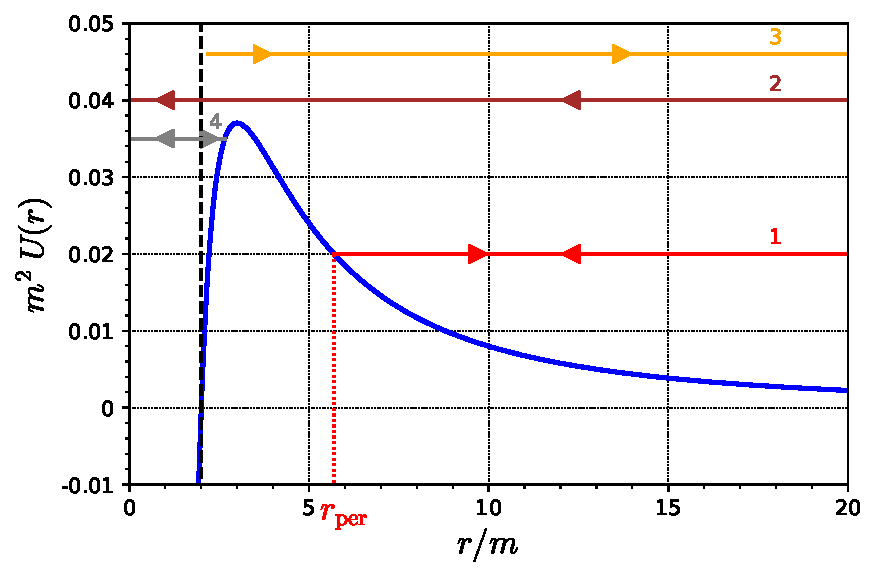
\includegraphics[width=0.8\textwidth]{ges_eff_pot_null.pdf}}
\caption[]{\label{f:ges:eff_pot_null} \footnotesize
Effective potential $U(r)$ (rescaled by $m^2$ to make it dimensionless)
governing the $r$-part of the
motion along a null geodesic in
Schwarzschild spacetime [Eq.~(\ref{e:ges:eff_pot_null})].
The vertical dashed line marks $r=2m$, i.e. the
location of the event horizon. The horizontal lines marked ``1'' to ``4''
correspond to the $r$-motion of four null geodesics,
the trajectories of which in the equatorial plane $\th=\pi/2$
are depicted in Fig.~\ref{f:ges:null_geod}.}
\end{figure}

\begin{figure}
\centerline{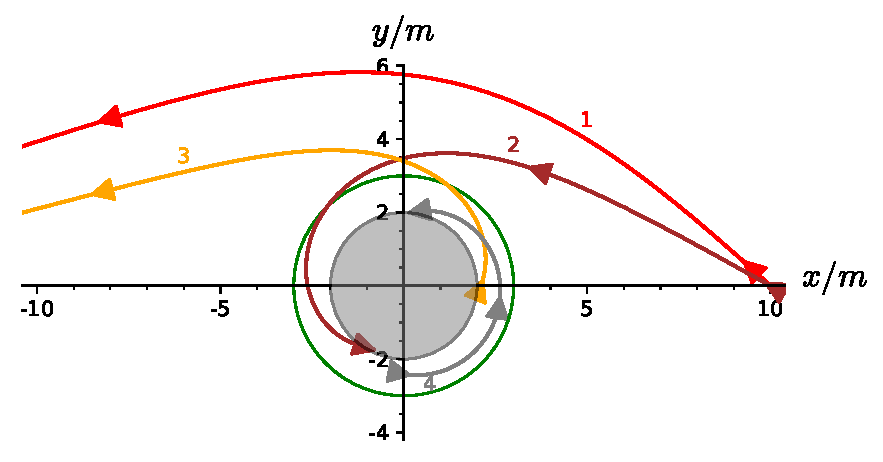
\includegraphics[width=0.8\textwidth]{ges_null_geod.pdf}}
\caption[]{\label{f:ges:null_geod} \footnotesize
Selected null geodesics in the equatorial plane of Schwarzschild spacetime,
plotted in terms
of the coordinates $(x,y) := (r\cos\ph, r\sin\ph)$, with the black hole
region $r<2m$ depicted as a grey disk.
The green geodesic is the photon circular orbit at $r=3m$.
The red geodesic (label ``1'') starts at $r_0=10 m$, $\ph_0=0$, with
the impact parameter $b = 7.071 \, m > b_{\rm crit}$ ($b^{-2} = 0.02\, m^{-2}$).
The brown geodesic (label ``2'') starts at $r_0=10 m$, $\ph_0=0$ with $b = 5 m < b_{\rm crit}$ ($b^{-2} = 0.04\, m^{-2}$).
The orange geodesic (label ``3'') starts outward at $r_0=2.1 m$, $\ph_0=0$ with $b = 4.663 m$ ($b^{-2} = 0.046\, m^{-2}$).
The grey geodesic (label ``4'') starts outward at $r_0=2.4 m$, $\ph_0=-\pi/2$ with $b = 5.345 m$ ($b^{-2} = 0.035\, m^{-2}$).
The $r$-motion of these four gedeosics is depicted in
Fig.~\ref{f:ges:eff_pot_null}.}
\end{figure}

The effective potential $U(r)$ is plotted in Fig.~\ref{f:ges:eff_pot_null}.
It has no minimum and a maximum at $r=3m$, which is
\be \label{e:ges:U_max}
    U_{\rm max} = \frac{1}{27m^2} .
\ee
This extremum is a stationary position in $r$: it corresponds thus to a circular
orbit, usually called the \defin{photon orbit}\index{photon!orbit}\index{orbit!photon --}.
The set of all photon orbits (one per choice of equatorial plane) is often
called the \defin{photon sphere}\index{photon!sphere}\index{sphere!photon --}.
However, since it corresponds to a maximum of the effective potential, the circular
orbit at $r=3m$ is an unstable orbit. So one should not imagine that a
Schwarzschild black hole is surrounded by a spherical shell of photons...


\subsection{Radial behaviour of null geodesics}

For the sake of concreteness, in this section and the remaining ones, we
refer to the massless particle $\mathscr{P}$ as a ``photon''. In most applications, in
particular the astrophysical ones, $\mathscr{P}$ will indeed be a photon.
But one shall keep in mind that all results are valid for any other massless
particle.

Since the effective potential
$U(r)$ has no minimum, it does not offer any potential well,
as it is clear from Fig.~\ref{f:ges:eff_pot_null}. This is in sharp contrast
with the effective potential $V_\ell(r)$ for massive particle
(compare Fig.~\ref{f:ges:eff_pot_bound}). Hence there are no bound orbits
for photons\footnote{unless one counts as ``bound'' a worldline that terminates in the
black hole region}.

We can infer various types of photon worldlines from Fig.~\ref{f:ges:eff_pot_null}.
In view of the ``first integral'' (\ref{e:ges:dot_r_square_null_b}),
each photon worldline can be represented by a horizontal line of ordinate
$b^{-2}$ in this figure, which must lie above the curve $U(r)$
by the positive quantity $({\D r}/{\D\tilde{\lambda}})^2$. The region under the curve
$U(r)$ is thus excluded.

For an initially inward photon, i.e. a photon emitted with ${\D r}/{\D\tilde{\lambda}} < 0$
from a position $r=r_{\rm em}$, there are
two possibilities, depending on the values of $r_{\rm em}$ and
of the impact parameter $b$:
\begin{itemize}
\item if $r_{\rm em} > 3 m$ and $b$ is large enough to fulfil $b^{-2} < U_{\rm max}$
(e.g. trajectory no.~1 in Fig.~\ref{f:ges:eff_pot_null}), the photon
``bounces'' on the potential barrier constituted by $U(r)$
at some minimal value  $r_{\rm per}$ of $r$ --- the \defin{periastron}\index{periastron},
which is given by  $U(r_{\rm per}) = b^{-2}$, or equivalently by
\be \label{e:ges:r_per_null}
  r_{\rm per}^3 - b^2\, r_{\rm per} + 2 m b^2 = 0, \quad r_{\rm per} > 3 m.
\ee
Equation~(\ref{e:ges:dot_r_square_null_b})
implies then
\be
    \left. \frac{\D r}{\D\tilde{\lambda}} \right| _{r = r_{\rm per}} = 0 .
\ee
Actually, $\D r / \D\tilde{\lambda}$ changes sign at $r = r_{\rm per}$ and
the photon subsequently moves away from the black hole for ever (cf. geodesic
no.~1 in Fig.~\ref{f:ges:null_geod}). We may call
such a worldline a scattering trajectory.
\item if $r_{\rm em} < 3 m$ (e.g. trajectory
no.~4 in Fig.~\ref{f:ges:eff_pot_null}) or $b$ is small enough to fulfil $b^{-2} > U_{\rm max}$ ((e.g. trajectory
no.~2 in Fig.~\ref{f:ges:eff_pot_null}) the photon
is not halted by the potential barrier constituted by $U(r)$. It then reaches arbitrary
small values of $r$ and is eventually absorbed by the black hole ($r < 2m$)
(cf. geodesic no.~2 in Fig.~\ref{f:ges:null_geod}).
\end{itemize}

For an initially outward photon, i.e. a photon emitted with ${\D r}/{\D\tilde{\lambda}} > 0$,
one has necessarily $r_{\rm em}>2m$ according to the result obtained in Sec.~\ref{s:ges:eq_to_be_solved}
and there are then two possible outcomes:

\begin{itemize}
\item if $r_{\rm em} > 3 m$ (e.g. trajectory
no.~1 in Fig.~\ref{f:ges:eff_pot_null}) or
$b$ is small enough to fulfil $b^{-2} > U_{\rm max}$ (e.g. trajectory
no.~3 in Figs.~\ref{f:ges:eff_pot_null}), the photon escapes to infinity
(cf. geodesic no.~3 in Fig.~\ref{f:ges:null_geod});
\item if $2m < r_{\rm em} < 3 m$ and $b^{-2} < U_{\rm max}$ (e.g. trajectory
no.~4 in Fig.~\ref{f:ges:eff_pot_null}), the photon ``bounces'' on the left
side of the potential barrier, reaching a maximal value of $r$
--- the \defin{apoastron}\index{apoastron},
which is given by  $U(r_{\rm apo}) = b^{-2}$, or equivalently by
\be \label{e:ges:r_apo_null}
   r_{\rm apo}^3 - b^2\, r_{\rm apo} + 2 m b^2 = 0, \quad r_{\rm apo} < 3 m.
\ee
The photon moves subsequently towards the black hole and
is absorbed by it (cf. geodesic no.~4 in Fig.~\ref{f:ges:null_geod}).
\end{itemize}

The critical value of the impact parameter separating the cases discussed
above is determined by $b_{\rm crit}^{-2} = U_{\rm max}$.
Given the value (\ref{e:ges:U_max}) of $U_{\rm max}$, we get
\be \label{e:ges:b_crit}
    \encadre{b_{\rm crit} = 3\sqrt{3} \, m \simeq 5.196152\, m }.
\ee

It follows from the above discussion that
\begin{greybox}
Along any null geodesic of Schwarzschild spacetime, the areal coordinate $r$
either is a monotonic function or has a single turning point. In the latter case,
if the turning point corresponds to a minimum of $r$ (a periastron, which can occur
only for $r>3m$), the null geodesic escapes to infinity, while if the turning
point corresponds to a maximum of $r$ (an apoastron, which can occur only for $2m<r<3m$), the
null geodesic terminates at the central singularity in $r=0$.
\end{greybox}
Note that for $r<2m$, i.e. in the black hole region, $r$
is always a monotonic function, since it has been demonstrated in
Sec.~\ref{s:ges:eq_to_be_solved} that $r(\tilde{\lambda})$ is scrictly
decreasing. The impossibility of a turning point for $r<2m$ can also be
graphically inferred from Fig.~\ref{f:ges:eff_pot_null}, which shows
that the effective potential $U(r)$ is negative for $r<2m$,
preventing the turning point condition $U(r) = b^{-2}$ to hold.

\begin{figure}
\centerline{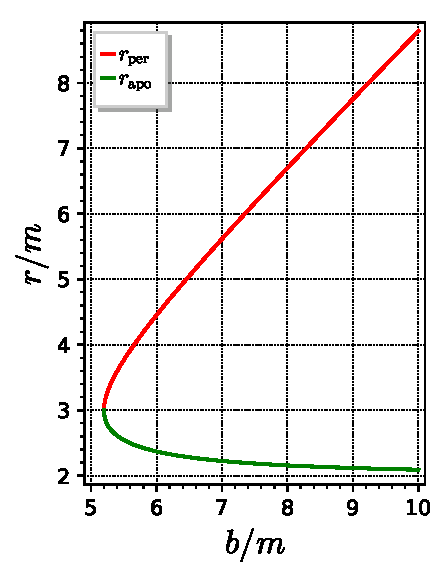
\includegraphics[width=0.4\textwidth]{ges_null_per_apo.pdf}}
\caption[]{\label{f:ges:null_per_apo} \footnotesize
Radial coordinate of the periastron, $r_{\rm per}$, and of the apoastron,
$r_{\rm apo}$, along a null geodesic with $b > b_{\rm crit} \simeq 5.196\, m$.
Note that a given null geodesic has either a periastron or an apoastron, but not
both.}
\end{figure}


For $b > b_{\rm crit}$, the explicit expression of the periastron radius
$r_{\rm per}$ (or the apoastron radius $r_{\rm apo}$)
is obtained by solving the cubic equation (\ref{e:ges:r_per_null})
(or (\ref{e:ges:r_apo_null}), which is the same cubic equation, except for
the range of the solution). Fortunately Eq.~(\ref{e:ges:r_per_null})
is a depressed\footnote{A \emph{depressed} cubic equation is a polynomial equation
of the type $x^3 + p x + q = 0$.} cubic equation, which makes
it simpler to solve. For $b > b_{\rm crit}$, its determinant is positive, which
implies that it admits three distinct real roots. Two of them are positive
and are precisely $r_{\rm per}$ and $r_{\rm apo}$. The third root is negative,
since the product of the roots is $-2mb^2 < 0$; it has therefore no
physical significance. The roots of the generic depressed cubic
equation $x^3 + p x + q = 0$ can be expressed via Viète's formulas:
\be
    x_k = 2 \sqrt{-\frac{p}{3}} \cos \left[ \frac{1}{3}\,  \mathrm{arccos}\left(
        \frac{3 q}{2 p} \sqrt{-\frac{p}{3}} \right) + \frac{2 k\pi}{3} \right],
        \qquad k \in \{0, 1, 2\} .
\ee
In the present case, $p= - b^2$ and $q = 2 m b^2$,
and $r_{\rm per}$ (resp. $r_{\rm apo}$) corresponds to $k=0$
(resp. $k=2$), so that we obtain
\be \label{e:ges:sol_r_per}
    r_{\rm per} = \frac{2 b}{\sqrt{3}} \cos\left[\frac{\pi}{3}
        - \frac{1}{3} \, \mathrm{arccos}\left(\frac{b_{\rm crit}}{b}\right) \right] .
\ee
\be \label{e:ges:sol_r_apo}
    r_{\rm apo} = \frac{2 b}{\sqrt{3}} \cos\left[\frac{5\pi}{3}
        - \frac{1}{3} \, \mathrm{arccos}\left(\frac{b_{\rm crit}}{b}\right) \right] .
\ee
As a check, we notice that for $b\gg b_{\rm crit}$, Eq.~(\ref{e:ges:sol_r_per})
yields $r_{\rm per} \simeq 2b/\sqrt{3} \cos\left(\pi/3 -1/3 \times \pi/2 \right)
\simeq 2b/\sqrt{3} \cos(\pi/6) \simeq b$, as expected.

The variation of $r_{\rm per}$ and $r_{\rm apo}$ with $b$ is plotted
on Fig.~\ref{f:ges:null_per_apo}. Note that $r_{\rm per} = r_{\rm apo} = 3 m$
(the photon orbit) at the limit $b = b_{\rm crit}$.



\subsection{Angular behaviour of null geodesics}

Let us first recall the generic property of causal geodesics in Schwarzschild
spacetime established in Sec.~\ref{s:ges:eq_to_be_solved} : the azimuthal
angle coordinate $\ph$ has no turning point: it is either always increasing
towards the future
($L>0$) or always decreasing towards the future ($L<0$). This is clear on
Eq.~(\ref{e:ges:dot_ph_null_b}) above, which implies obviously
$\D\ph/\D\tilde{\lambda} > 0$, with $\tilde{\lambda}$ increasing (resp. decreasing)
towards the future for $L>0$ (resp. $L<0$).

By combining Eqs.~(\ref{e:ges:dot_ph_null_b}), (\ref{e:ges:dot_r_square_null_b})
and (\ref{e:ges:eff_pot_null}), we get
\be \label{e:ges:dphi_dr_null}
    \frac{\D\ph}{\D r} = \pm \frac{1}{r^2} \left( \frac{1}{b^2}
        - \frac{1}{r^2} \left( 1 - \frac{2m}{r} \right) \right) ^{-1/2} .
\ee
This equation governs the trace of null geodesics on the equatorial plane
$\th=\pi/2$.

\begin{figure}
\begin{tabular}{cc}
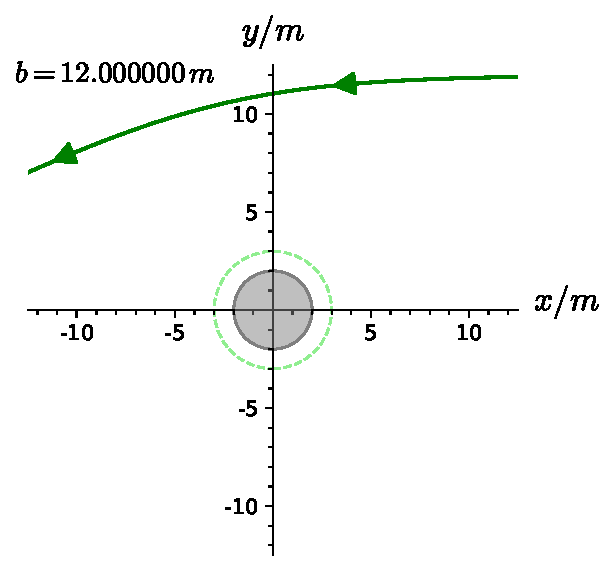
\includegraphics[width=0.48\textwidth]{ges_null_b_12_000000.pdf} &
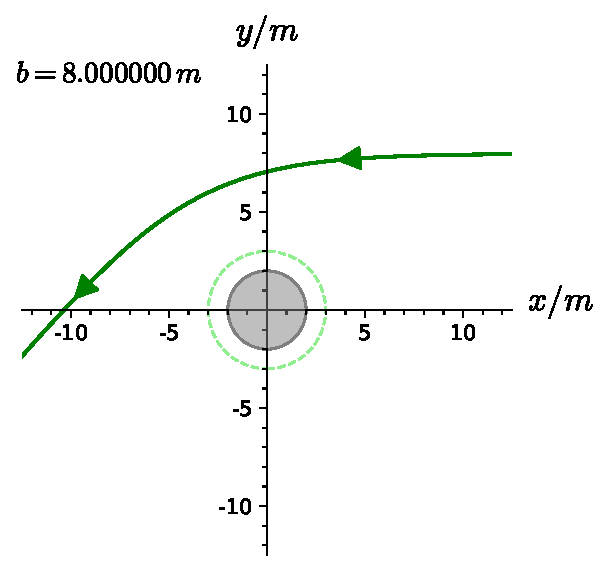
\includegraphics[width=0.48\textwidth]{ges_null_b_8_000000.pdf} \\
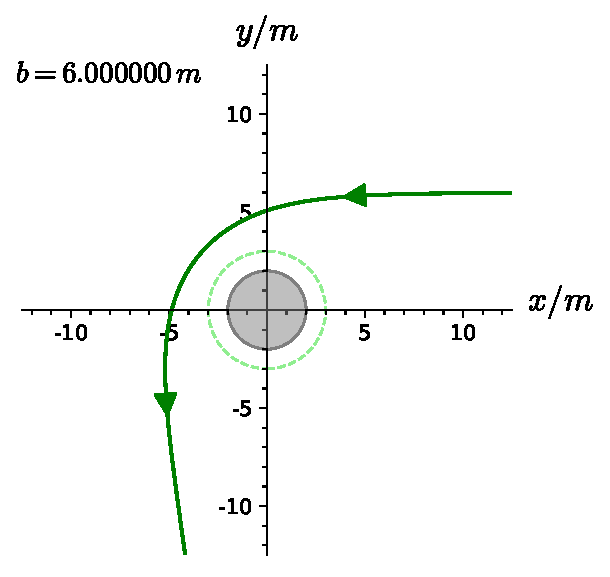
\includegraphics[width=0.48\textwidth]{ges_null_b_6_000000.pdf} &
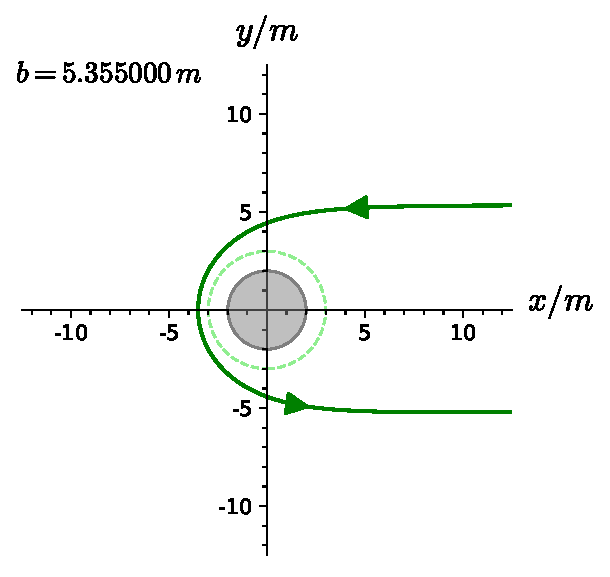
\includegraphics[width=0.48\textwidth]{ges_null_b_5_355000.pdf}
\end{tabular}
\caption[]{\label{f:ges:null_b1} \footnotesize
Null geodesics in the equatorial plane of Schwarzschild spacetime,
plotted in terms of the coordinates $(x,y) := (r\cos\ph, r\sin\ph)$,
arising from $x\gg m$ with trajectories all initially parallel to the $x$-axis,
but differing by the value of the impact parameter $b$.
The grey disk marks the black hole
region $r<2m$, while the dashed green circle indicates the photon orbit
at $r=3m$.}
\end{figure}

\begin{figure}
\begin{tabular}{cc}
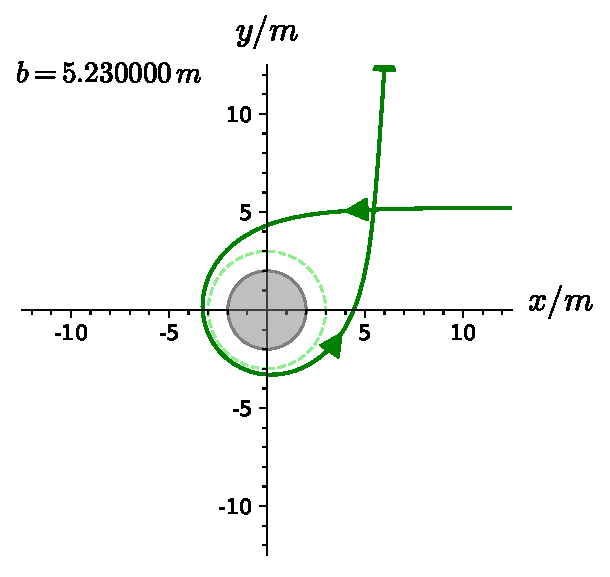
\includegraphics[width=0.48\textwidth]{ges_null_b_5_230000.pdf} &
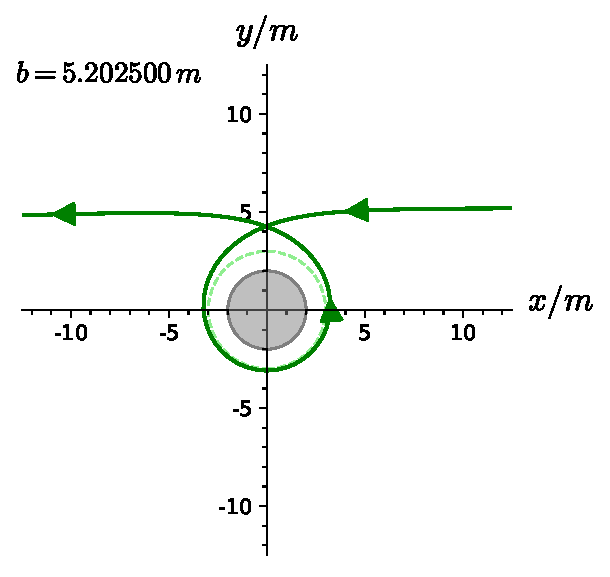
\includegraphics[width=0.48\textwidth]{ges_null_b_5_202500.pdf} \\
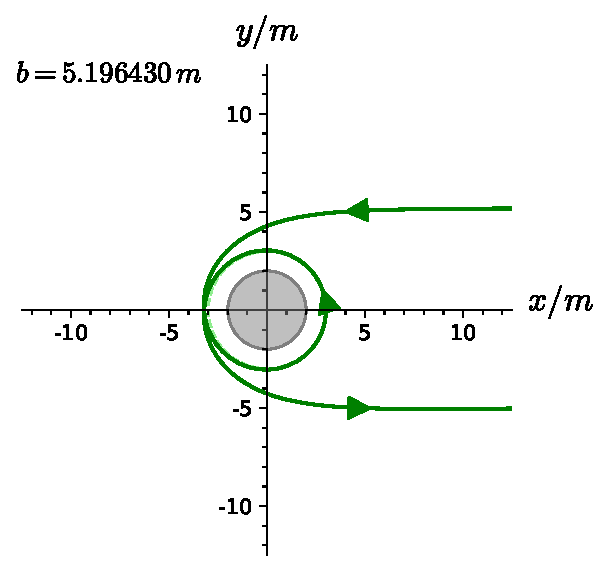
\includegraphics[width=0.48\textwidth]{ges_null_b_5_196430.pdf} &
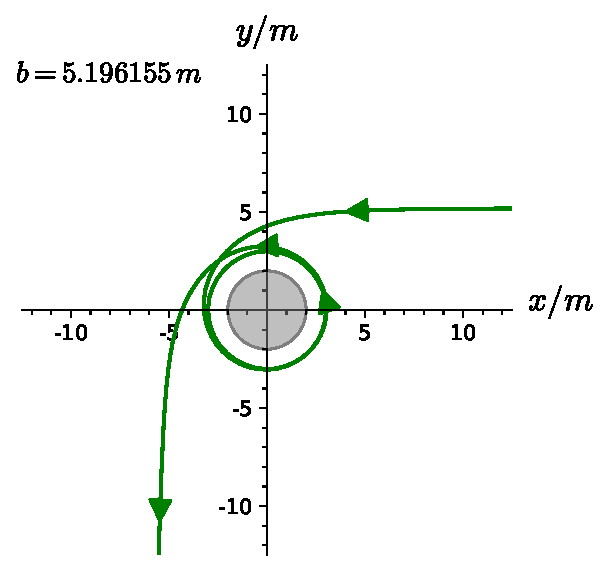
\includegraphics[width=0.48\textwidth]{ges_null_b_5_196155.pdf}
\end{tabular}
\caption[]{\label{f:ges:null_b2} \footnotesize
Same as Fig.~\ref{f:ges:null_b1} but for values of $b$ closer to
$b_{\rm crit} \simeq 5.196152\, m$.}
\end{figure}

Figures~\ref{f:ges:null_b1}-\ref{f:ges:null_b2} show such traces from null
geodesics coming from infinity along the
direction $\ph=0$, for various values of the
impact parameter $b$ decaying to $b_{\rm crit}$. All these geodesics, having
$b > b_{\rm crit}$, correspond to the case no.~1 in the effective potential
diagram of Fig.~\ref{f:ges:eff_pot_null}, i.e. they reach a periastron
before escaping to infinity. However, they differ by the number of turns
performed around the black hole. For $b=12 m$ (upper left panel of Fig.~\ref{f:ges:null_b1}),
the geodesic suffers only some small bending; this is nothing but the standard
\defin{deflection of light}\index{deflection of light} by massive bodies in
general relativity. For $b=8 m$ and $6 m$, the bending is more pronounced,
exceeding $\Delta\ph = \pi/2$ for $b=6 m$. For $b=5.355 m$ (lower right panel of Fig.~\ref{f:ges:null_b1}), the bending is such that the photon goes back in the direction
from which it was coming.

When the impact parameter becomes even closer to the critical value (\ref{e:ges:b_crit}),
the null geodesic starts to wind around the black hole before escaping
to infinity (Fig.~\ref{f:ges:null_b2}). Note that the winding is taking place
almost at the photon circular orbit ($r=3m$). That after a few turns the null geodesic
departs to infinity corroborates the fact that the photon orbit is unstable
(cf. Sec.~\ref{s:ges:null_eff_pot}).

The total change in $\ph$ along the null geodesic
is obtained by integrating Eq.~(\ref{e:ges:dphi_dr_null}), when $r$ varies
from $+\infty$ (the ``far away'' emission) to $r_{\rm per}$, and then when
$r$ varies from $r_{\rm per}$ to $+\infty$ (the ``far away'' reception).
Assuming $L>0$, so that $\ph$ increases towards the future, one must select
the $-$ sign in the r.h.s. of Eq.~(\ref{e:ges:dphi_dr_null}) for the first part
and the $+$ sign for the second part. Hence
\bea
    \Delta \ph &=& - \int_{+\infty}^{r_{\rm per}} \frac{1}{r^2} \left( \frac{1}{b^2}
        - \frac{1}{r^2} \left( 1 - \frac{2m}{r} \right) \right) ^{-1/2} \D r
    + \int_{r_{\rm per}}^{+\infty}  \frac{1}{r^2}\left( \frac{1}{b^2}
        - \frac{1}{r^2} \left( 1 - \frac{2m}{r} \right) \right) ^{-1/2} \D r \nonumber \\
        & = & 2 \int_{r_{\rm per}}^{+\infty}  \frac{1}{r^2}\left( \frac{1}{b^2}
        - \frac{1}{r^2} \left( 1 - \frac{2m}{r} \right) \right) ^{-1/2} \D r
\eea
Via the change of variable
\be
    u := \frac{m}{r}
\ee
we can transform the integral into
\be
    \Delta\ph = 2 \int_0^{u_{\rm per}} \frac{\D u}{\sqrt{2 u^3 - u^2 + (m/b)^2}} ,
\ee
with $u_{\rm per} := m/r_{\rm per}$.
This integral can be evaluated by means of elliptic functions (see e.g. Ref.~\cite{Lumin79, FroloZ11}
for details). However, we can understand the winding around the photon circular orbit
observed in Figs.~\ref{f:ges:null_b1}-\ref{f:ges:null_b2}
when $b$ is close to $b_{\rm crit}$
without the explicit form.
Indeed the roots of the cubic polynomial
$2 u^3 - u^2 + (m/b)^2$  are nothing but $u_{\rm per} := m/r_{\rm per}$,
$u_{\rm apo} := m/r_{\rm apo}$ and $u_{\rm neg} := m/r_{\rm neg}$
with $r_{\rm per}$ given by Eq.~(\ref{e:ges:sol_r_per}), $r_{\rm apo}$
given by Eq.~(\ref{e:ges:sol_r_apo}) and $r_{\rm neg}$ is the negative root
of the polynomial $r^3 - b^2 r + 2 m b^2$. We thus can write
\be
    \Delta\ph = \sqrt{2} \int_0^{u_{\rm per}}
    \frac{\D u}{\sqrt{(u_{\rm per} - u )(u_{\rm apo} - u)(u - u_{\rm neg})}} .
\ee


\subsection{Black hole shadow}


\begin{hist}
Darwin \cite{Darwi59}, Synge \cite{Synge66}, Bardeen \cite{Barde73}
\end{hist}














